% Project report: Agentic AI Procurement Solution
% Fr. C. Rodrigues Institute of Technology, Vashi -- report template by Dr. Smita Dange.
% Every package and style lives in this file; the other .tex files hold content only.
% Build: pdflatex (Overleaf default), latexmk -pdf main.tex, or tectonic main.tex

\documentclass[12pt]{report}
\usepackage{graphicx}
\usepackage{geometry}
\usepackage{ragged2e}
\usepackage{titlesec}
\usepackage{fancyhdr}
\usepackage{tabularx}
\usepackage{array}
\usepackage{longtable}
\usepackage{amsmath,amssymb}
\usepackage{xcolor}
\usepackage{listings}
\usepackage[font=small,labelfont=bf]{caption}
\usepackage{hyperref}
% Cross-references stay black; links to papers and web pages are blue so
% that a reader can see they are clickable.
\definecolor{linkblue}{HTML}{1F4E9C}
\hypersetup{colorlinks=true, linkcolor=black, citecolor=black, urlcolor=linkblue}

\titleformat{\chapter}[display]
  {\normalfont\huge\bfseries\centering}
  {\chaptertitlename\ \thechapter}{24pt}{\Huge}
\geometry{verbose,a4paper,tmargin=15mm,bmargin=30mm,lmargin=30mm,rmargin=20mm}

% Header and footer
\geometry{headheight=15pt}
\setcounter{tocdepth}{3}
\setcounter{secnumdepth}{3}

\pagestyle{fancy}
\fancyhf{}
\rhead{Agentic AI Procurement Solution}
\lfoot{F.C.R.I.T, Vashi}
\rfoot{\thepage}
\renewcommand{\footrulewidth}{0.6pt}
\renewcommand{\headrulewidth}{1.pt}

% ---------------------------------------------------------------
% Tables: one style for every table in the report
% ---------------------------------------------------------------
\newcolumntype{L}[1]{>{\raggedright\arraybackslash}p{#1}}
\newcolumntype{C}[1]{>{\centering\arraybackslash}p{#1}}
\newcolumntype{Y}{>{\raggedright\arraybackslash}X}
\newcommand{\tablestyle}{\footnotesize\renewcommand{\arraystretch}{1.25}}
\setlength{\LTpre}{6pt}\setlength{\LTpost}{6pt}

% ---------------------------------------------------------------
% Figures: every diagram and chart is a separate file in figures/diagrams/
% (TikZ source + the built PDF that is included here). The report does not
% load TikZ, which keeps it within Overleaf's compile time limit. After
% editing a diagram, rebuild its PDF with figures/diagrams/build.sh.
% ---------------------------------------------------------------

% Code listings
\lstset{
  basicstyle=\ttfamily\scriptsize, columns=fullflexible, keepspaces=true,
  frame=single, rulecolor=\color{black!40}, framesep=4pt, xleftmargin=6pt, xrightmargin=6pt,
  numbers=left, numberstyle=\tiny\color{black!50}, numbersep=6pt,
  commentstyle=\color{black!55}\itshape, keywordstyle=\bfseries, stringstyle=\color{black!75},
  showstringspaces=false, breaklines=true, language=Python, captionpos=b,
}
\renewcommand{\lstlistingname}{Listing}
\captionsetup[lstlisting]{justification=raggedright,singlelinecheck=false}
\renewcommand{\bibname}{References}

\setlength{\emergencystretch}{2.5em}
\newcommand{\Rs}{Rs.\,}
\newcommand{\code}[1]{\texttt{\detokenize{#1}}}
% Something the team still has to fill in: printed in red. Search for \todo
% before submission; none should be left.
\newcommand{\todo}[1]{\textcolor{red}{\textbf{\mbox{TO-DO:}} #1}}

\begin{document}
\pagestyle{plain}
% Title Page

\begin{titlepage}
\thispagestyle{empty}
\begin{center}
{A Project Report}\\[0.2cm]
{On}\\[0.3cm]
{\LARGE\bfseries Agentic AI Procurement Solution}\\[0.8cm]

{\large
Submitted in partial fulfilment of the requirements of\\[0.2cm]
\textbf{University of Mumbai}\\[0.2cm]
For the Degree of\\[0.2cm]
\textbf{Bachelor of Engineering}\\
\textit{in}\\
\textbf{COMPUTER ENGINEERING}\\[0.5cm]

\textit{Submitted by}\\[0.2cm]
\textbf{More Anjali Dinesh}\\
\textbf{Sankaye Vaidehi Jagdeep}\\
\textbf{Sawant Niraj Ravindra}\\
\textbf{Shete Anooj}\\[0.6cm]

\textit{Supervised by}\\[0.1cm]
\textbf{Dr. Jyoti More}\\[0.1cm]
\textit{\&}\\[0.1cm]
\textbf{Mr. Alok Chilka}\\
\textbf{(External guide)}\\[0.4cm]


\includegraphics[width=3.6cm,height=3.6cm]{fcritlogo}\\[0.3cm]

\textbf{Department of Computer Engineering}\\[0.1cm]
\textbf{Fr. Conceicao Rodrigues Institute of Technology}\\
\textbf{An Autonomous Institute \& Permanently Affiliated to University of Mumbai}\\
\textbf{Sector 9A, Vashi, Navi Mumbai - 400703}\\[0.5cm]

\textbf{UNIVERSITY OF MUMBAI}\\
\textbf{2026--2027}
}
\end{center}
\end{titlepage}

\pagenumbering{roman}

% Approval Page

\begin{center}
{\LARGE\bfseries APPROVAL SHEET}

\vspace{1cm}
{\large This is to certify that the project entitled}\\[0.3cm]
{\Large\textsc{Agentic AI Procurement Solution}}\\[0.3cm]
{\large\bfseries Submitted by}\\[0.5cm]

{\Large
\begin{tabular}{cc}
\textbf{More Anjali Dinesh} & \textbf{1023207} \\
\textbf{Sankaye Vaidehi Jagdeep} & \textbf{1023239} \\
\textbf{Sawant Niraj Ravindra} & \textbf{1023240} \\
\textbf{Shete Anooj} & \textbf{1023250}
\end{tabular}}

\vspace{2cm}
\begin{tabular}{cc}
\begin{minipage}{0.42\textwidth}\centering\rule{5cm}{0.4pt}\\\textbf{Supervisor / Project Guide}\end{minipage} &
\begin{minipage}{0.42\textwidth}\centering\rule{5cm}{0.4pt}\\\textbf{Project Coordinator}\end{minipage}
\end{tabular}

\vspace{2.2cm}
\begin{tabular}{cc}
\begin{minipage}{0.42\textwidth}\centering\rule{5cm}{0.4pt}\\\textbf{Internal Examiner}\end{minipage} &
\begin{minipage}{0.42\textwidth}\centering\rule{5cm}{0.4pt}\\\textbf{External Examiner}\end{minipage}
\end{tabular}

\vspace{2.2cm}
\begin{tabular}{cc}
\begin{minipage}{0.42\textwidth}\centering\rule{5cm}{0.4pt}\\\textbf{Head of Department}\end{minipage} &
\begin{minipage}{0.42\textwidth}\centering\rule{5cm}{0.4pt}\\\textbf{Principal}\end{minipage}
\end{tabular}

\vspace{1.5cm}
\textbf{COLLEGE SEAL}

\vspace{2cm}
\begin{flushleft}
\textbf{Date :} \rule{4cm}{0.4pt}\\[0.4cm]
\textbf{Place :} \rule{4cm}{0.4pt}
\end{flushleft}
\end{center}

% Declaration Page

\begin{centering}
\large
{\LARGE\bf Declaration}\\
\end{centering}

% workaround for the inconsistent justify. If someone figures out the right way to strictly justify, let me know
\justify
We declare that this written submission for the B.E. degree, entitled
``{\bf Agentic AI Procurement Solution}'', represents our ideas in our own words, and that where others' ideas or words have been included, we have adequately cited and referenced the original sources. We also declare that we have adhered to all principles of academic honesty and integrity and have not misrepresented, fabricated, or falsified any ideas/data/fact/source in our submission. We understand that any violation of the above will cause disciplinary action by the institute and also evoke penal action from the sources which have thus not been properly cited or from whom permission has not been taken when needed.  \\ 

\vspace{3cm}
\hfill% move it to the right
\begin{tabular}[t]{l@{}}
\vspace{1cm}

{\textbf{Project Group Members:}} \\ 
\vspace{1cm}

1. More Anjali Dinesh, 1023207 \\
\noindent\rule{5cm}{0.10pt} \\
\\
\vspace{1cm}

2. Sankaye Vaidehi Jagdeep, 1023239 \\
\noindent\rule{5cm}{0.10pt} \\
\\
\vspace{1cm}

3. Sawant Niraj Ravindra, 1023240 \\
 \noindent\rule{5cm}{0.10pt}
\\
\vspace{1cm}


4. Shete Anooj, 1023250 \\
 \noindent\rule{5cm}{0.10pt}

\end{tabular}

%%%%%%%%%%%%%%%%%%%%%%%%%%%%%%%%%%%%IGNORE PLEASE !
%\begin{flushright} 
%\vspace{0.5in}
%\noindent\rule{4cm}{0.4pt} \\ (Signature)\\
%\vspace{0.3in}
%\noindent\rule{4cm}{0.4pt} \\ (Name of the Student)
%\end{flushright}
%\vspace{0.5cm}
%{\bf Date:} \\
%%%%%%%%%%%%%%%%%%%%%%%%%%%%%%%%%%%%


%% End of Declaration Page


\newpage
\addcontentsline{toc}{chapter}{Abstract}
% Abstract
\vspace{1in}
\chapter*{Abstract}

IT procurement covers the purchase, licensing, renewal and risk assessment of hardware, software and SaaS services. In many organisations it is still handled through e-mail, spreadsheets and separate tools, which leads to slow approvals, duplicate payments, unused licences, missed contract renewals and weak visibility of vendor risk. Existing techniques such as OCR, rule-based extraction, approval workflows and machine learning usually address one stage of the procurement cycle in isolation.

This report presents an Agentic AI-based IT Procurement Intelligence Platform built as an event-driven system of four cooperating agents: Document and Vendor Intelligence, Approval and Inventory Intelligence, Contract and Risk Analysis, and a Platform agent that provides authentication, business rules, notifications and a conversational assistant. Each agent is an independent FastAPI service that reacts to events on a Kafka-compatible bus (Redpanda), decides with rules or trained models, and publishes its result through a transactional outbox; long-running steps run as Temporal workflows, and decisions that are uncertain or sensitive are handed to a person.

Uploads are scanned with ClamAV and read with pdfplumber, Docling or PaddleOCR. A TF-IDF and logistic-regression classifier, regular-expression field extraction and an optional LayoutLMv3 cross-check produce a confidence-scored record, and records below a confidence of 0.8 go to a review queue. Vendors are matched by normalised fuzzy name, onboarding validates GSTIN check digits and IFSC codes, bank details require a second person's verification, and duplicate invoices are flagged. Requests follow spend-tier approval chains with SLA escalation and Redis-locked stock reservation; an Isolation Forest with SHAP explanations proposes licence reclaims after a grace period. Contracts are generated from templates, signed in the application, and read by a Legal-BERT model fine-tuned on CUAD, and vendors carry a Random Forest risk score with hard overrides for a cancelled GSTIN or a sanctions match, monitored for drift with the Population Stability Index.

On synthetic data, the shipped classifier reached a macro-F1 of 1.0 against 0.912 for a keyword baseline; Legal-BERT reached F1 scores of 0.85, 0.80 and 0.91 on three clause types of the CUAD test split, against 0.50, 0.19 and 0.02 for rules; the licence-anomaly model reached a ROC-AUC of 0.954; and the risk model reached a ROC-AUC of 0.715 against a ceiling of 0.739 set by its label noise. Field extraction was complete on text PDFs but reached only 49\% on photographed images. The implementation passes 823 service unit tests and four end-to-end suites through the gateway. All datasets are synthetic, so these figures compare methods rather than predict performance on an organisation's real documents.

\vspace{0.5cm}
\noindent\textbf{Keywords:} agentic AI, IT procurement, event-driven architecture, document intelligence, human-in-the-loop, vendor risk, anomaly detection, contract analysis.


\tableofcontents
\newpage

\addcontentsline{toc}{chapter}{List of Figures}
\listoffigures
\newpage

\addcontentsline{toc}{chapter}{List of Tables}
\listoftables
\newpage

\renewcommand{\lstlistlistingname}{List of Listings}
\addcontentsline{toc}{chapter}{List of Listings}
\lstlistoflistings
\newpage

\pagenumbering{arabic}
\pagestyle{fancy}
% Chapter 1 Introduction

\chapter[Introduction]{\centering Introduction}\label{chap1}
\newpage

\section{Background}
IT procurement is an important part of an organisation's operations because it covers the acquisition and management of hardware, software licences, SaaS subscriptions and related services. The process runs through several stages: identifying a vendor, processing its documents, obtaining approval, managing inventory, handling the contract and assessing vendor risk. In many organisations these activities are spread across e-mail, spreadsheets, invoices and separate systems, which makes it hard to keep a consistent, current view of procurement. Approvals are delayed, purchases are duplicated, licences go unused, contracts are difficult to track and vendor-related risks grow unnoticed. Automation and artificial intelligence offer a way to make these activities faster and more reliable.

\section{Motivation}
The project is motivated by the time spent on manual procurement work and the lack of transparency and control that results from it. Employees verify documents, review vendor details, chase approvals, check stock and licence utilisation, and keep track of contract renewals. These tasks become error-prone as volumes grow, and some of the resulting errors, such as paying a fraudulent change of bank details, are costly. A system that automates the routine steps, links the stages of the procurement cycle and asks a person only when a decision is uncertain or sensitive would be of clear benefit. The project therefore implements a set of special-purpose software agents for document processing, vendor matching, approvals, inventory and licence analysis, contract management and risk detection.

\section{Aim and Objectives}

\subsection{Aim}
To develop an Agentic AI-based IT Procurement Intelligence Platform that integrates, automates and intelligently manages the major activities of the IT procurement lifecycle while keeping human oversight of critical decisions.

\subsection{Objectives}
\begin{itemize}
  \item To process procurement documents such as purchase orders, invoices and quotations, and extract their key fields with a confidence score for each result.
  \item To match vendors against existing records, validate their tax and bank identifiers, and detect duplicate vendors and duplicate invoices.
  \item To automate approval workflows based on spend tiers, an approval-authority matrix, SLA deadlines and inventory availability, with escalation when an approver does not respond.
  \item To detect under-used software licences with an anomaly-detection model and propose their reclamation under human control.
  \item To support contract management by generating contracts, collecting signatures, extracting renewal-related clauses and issuing renewal reminders.
  \item To assess vendor risk with a machine learning model, explain each score, and monitor the model for drift.
  \item To provide shared platform services: authentication, role-based access control, configurable business rules, notifications, monitoring and audit logging.
  \item To keep humans involved in low-confidence results and in critical decisions such as changes to vendor payment details.
\end{itemize}

\section{Problem Statement}
IT procurement involves collecting procurement documents, verifying vendor information, processing invoices and quotations, obtaining approvals, managing software licences, monitoring contracts and assessing vendor risk. These activities are often handled through several systems and manual processes, which causes delays, duplicate records, wasted resources and limited visibility across the procurement lifecycle.

Traditional procurement systems mainly record transactions; they do little to analyse procurement data or to support decisions. Identifying duplicate vendors or invoices, detecting under-used licences, tracking renewals and assessing vendor risk therefore take significant manual effort. At the same time, automated decisions made without a measure of confidence and without human oversight can lead to incorrect procurement actions.

There is therefore a need for an integrated solution that automates routine procurement activities, analyses the relevant data, supports approval decisions and monitors procurement risk. The proposed platform addresses this need by combining document processing, vendor intelligence, workflow automation, licence management, contract monitoring, risk scoring and human-in-the-loop controls in one system.

\section{Scope}
The platform covers the following activities of the IT procurement lifecycle:
\begin{itemize}
  \item \textbf{Procurement document processing:} receiving documents by upload, e-mail or a watched folder; scanning, parsing, classifying and extracting structured fields from purchase orders, invoices and quotations.
  \item \textbf{Vendor intelligence:} matching extracted vendor names against existing records, onboarding vendors with GSTIN and IFSC validation, and holding new or changed bank details for verification by a second user.
  \item \textbf{Invoice checks:} flagging likely duplicate invoices and matching invoices line by line against the purchase request.
  \item \textbf{Approval workflow automation:} routing purchase requests through spend-tier approval chains with SLA timers, reminders, escalation and inventory reservation.
  \item \textbf{Software licence management:} scoring licence usage for anomalies and creating reclaim requests that a person approves after a grace period.
  \item \textbf{Contract management:} generating contracts from templates, signing them in the application, extracting renewal type, notice period and end date, and scheduling renewal reminders.
  \item \textbf{Vendor risk assessment:} scoring vendors with a machine learning model and hard-override rules, listing the contributing factors, and monitoring the model for drift.
  \item \textbf{Shared platform services:} authentication, role-based access control, business rules editable at run time, e-mail notifications, audit logging, metrics, centralised logs and a conversational assistant.
  \item \textbf{Human-in-the-loop decision making:} routing low-confidence documents, payment-detail changes, reclaims and high-risk signatures to authorised users.
\end{itemize}
The platform is a decision-support and workflow-automation system; it does not replace human decision-makers in critical procurement activities. Payment execution, ERP integration and production deployment are outside the scope (Section~\ref{sec:scope3}).

\section{Report Outline}
This report is organised into six chapters. Chapter~\ref{chap1}, \textbf{Introduction}, presents the background, motivation, aim and objectives, problem statement and scope. Chapter~\ref{chap2}, \textbf{Study of the System}, reviews the techniques relevant to each part of the system and compares related research. Chapter~\ref{chap3}, \textbf{Proposed System}, describes the problem, the scope and the proposed platform: its architecture, agents, document pipeline, event flow and technology stack. Chapter~\ref{chap4}, \textbf{Design of the System}, covers requirement engineering, the lifecycle model, UML diagrams and data-flow diagrams, cost analysis, hardware and software requirements, and the system architecture. Chapter~\ref{chap5}, \textbf{Result and Discussion}, presents screenshots of the implemented system, its main logic, the testing performed and the evaluation of its models. Chapter~\ref{chap6}, \textbf{Conclusion and Future Scope}, summarises the outcomes, limitations and possible extensions. The report ends with references and appendices covering the project timeline, SDG mapping, complex engineering problem evaluation and project outcomes.

% Chapter 2: Study of the System

\chapter{Study of the System} \label{chap2}
\newpage

Procurement documents---purchase orders, invoices and quotations---arrive by e-mail, through vendor portals or as scans, rarely in the same layout twice, and are often still keyed in by hand. Contracts are followed up in spreadsheets, vendors are vetted once at onboarding, and licences are checked with an inactivity rule. The result is data-entry errors, duplicate payments, unverified vendors, silent renewals and idle licences, as well as exposure to Business Email Compromise (BEC), in which an attacker posing as a supplier has its bank details changed because nobody verifies the request independently.

Each agent of the proposed platform draws on a different set of methods, so this chapter reviews several techniques rather than one. It contrasts traditional practice with automated alternatives, reviews the techniques for each sub-problem together with the choice made in this project, compares ten related works and five commercial procurement platforms, and identifies the gap the project addresses.

\section{About the Technique}
Traditional procurement processing rests on four habits. The first is manual or template-based data entry: staff key in invoice and purchase-order details, or an OCR template is built for each vendor's layout. The second is static approval rules, where a request follows a fixed chain with no deadline, no escalation and no awareness of remaining stock. The third is periodic vendor review, which in practice often means one questionnaire at onboarding. The fourth is the flat-threshold licence audit, in which a seat is flagged when nobody has logged in for a fixed number of days. These habits work at small volumes but break down as an organisation grows; Table~\ref{tab:traditional} summarises where each struggles.

\begin{table}[H]
\centering\tablestyle
\caption{Traditional procurement practices and their shortcomings}\label{tab:traditional}
\begin{tabularx}{\textwidth}{|L{0.19\textwidth}|L{0.27\textwidth}|Y|}
\hline
\textbf{Area} & \textbf{Traditional approach} & \textbf{Shortcoming} \\ \hline
Data capture & Manual entry and per-vendor templates & Slow and error-prone; templates break whenever a vendor changes its layout. \\ \hline
Vendor verification & Manual lookup and e-mail confirmation & Vulnerable to BEC fraud; duplicate vendor records accumulate. \\ \hline
Approvals & E-mail chains and fixed rules & No SLA timers or escalation; overlapping requests can claim the same stock. \\ \hline
Licence management & Fixed inactivity threshold & Ignores usage patterns and wrongly flags seasonal or weekend dips. \\ \hline
Contract tracking & Calendar reminders & Notice periods are missed, resulting in unintended automatic renewals. \\ \hline
Risk assessment & One-time questionnaire & Becomes outdated; misses later events such as a cancelled tax registration or a sanctions listing. \\ \hline
\end{tabularx}
\end{table}

These gaps motivate an automated, event-driven approach, but not one that hands every decision to a model. Pretrained components handle perception-heavy work such as reading page layouts and contract language; small models are trained where a task is specific to this project (document classification, licence anomalies and vendor risk), and each trained model is kept only if it beats a simple baseline on held-out data; and plain rules remain wherever certainty and auditability matter more than flexibility, such as spend-tier routing, sanctions overrides and dual control of bank details.

\section{Various Available Techniques}

\subsection{Document Intelligence}
Template and regular-expression approaches are fast and predictable but brittle when vendors change layouts. OCR engines such as Tesseract~\cite{smith2007tesseract} and PaddleOCR~\cite{cui2025paddleocr} recover text from scanned pages but lose table structure. Layout-aware parsers such as Docling~\cite{auer2024docling} recover reading order and tables, although they are not tuned to invoices. Multimodal transformers of the LayoutLM family~\cite{xu2020layoutlm,huang2022layoutlmv3} give the best results on forms and invoices but need labelled data and more compute.

\emph{Choice in this project.} PDFs with a usable text layer are read directly with pdfplumber; scanned PDFs go through Docling and its bundled OCR engine; images are read by PaddleOCR after deskewing and limited upscaling. PaddleOCR's native engine aborted the host process on some platform and version combinations, so it runs in an isolated subprocess with a time limit rather than in the worker itself. Fields are then extracted with regular expressions. When the LayoutLMv3 weights are installed, the model reads every document a second time as an independent cross-check (a disagreement forces human review) and replaces the OCR reading of an image whose OCR quality falls below 0.5.

\subsection{Document Classification}
TF-IDF features with logistic regression are light, fast to train and easy to inspect, which suits a small number of document classes. Transformer classifiers such as BERT have a higher ceiling but need more data and compute than this task justifies. A weighted keyword classifier, which scores title phrases such as ``tax invoice'' or ``purchase order'', needs no training data but depends on the vocabulary it is given.

\emph{Choice in this project.} A TF-IDF (character 2--5-grams) and logistic-regression classifier labels each document as an invoice, purchase order, quotation or \emph{other} paperwork. It was trained and evaluated on a corpus of 1,260 generated documents that includes OCR-noise and missing-title variants, and was kept only because it beat the keyword classifier on validation data and on document kinds held out of training (Section~\ref{sec:eval}). The keyword classifier remains the fallback whenever the model is less than 60\% confident.

\subsection{Vendor Deduplication and Identity Verification}
Fuzzy name matching (rapidfuzz) tolerates spelling differences and corporate suffixes but can produce false matches on its own. Official identifiers are more reliable: an Indian GSTIN carries a check digit that can be validated offline, and an IFSC code can be looked up in a public bank directory, while live registry lookups are limited by API quotas.

\emph{Choice in this project.} Extracted vendor names are normalised and matched with a fuzzy ratio threshold of 88. Vendor onboarding validates GSTIN format and check digit and looks IFSC codes up in a public directory, flags names 70--87\% similar to an existing vendor as possible impostors, and never writes bank details directly: they become a pending change that a second finance or admin user must verify. Every upload is scanned with ClamAV, which is signature-based and therefore fast but offers no protection against zero-day threats.

\subsection{Workflow Orchestration and Concurrency Control}
Cron jobs and scripts are simple but not durable and handle deadlines poorly. Temporal offers durable timers, signals and replay, at the cost of a steeper learning curve. Redis or database locks stop two requests from claiming the same stock, but need careful failure handling. Kafka-compatible brokers~\cite{kreps2011kafka} provide decoupled, replayable events between services, provided that consumers are idempotent; and a transactional outbox~\cite{richardson2018microservices} ensures that an event is published if and only if the database change that caused it commits.

\emph{Choice in this project.} Temporal runs the approval, reclaim and renewal workflows; a short-lived Redis lock guards each stock reservation; Redpanda is the event bus; and events are written through a transactional outbox and consumed with retries and a dead-letter table.

\subsection{Usage Anomaly Detection and Explainability}
A flat inactivity threshold is transparent but flags seasonal and weekend dips by mistake. Isolation Forest~\cite{liu2008isolation} is unsupervised and efficient on tabular data, though it is sensitive to its contamination setting and gives no explanation of its own; SHAP~\cite{lundberg2017shap} supplies per-feature contributions at some extra cost.

\emph{Choice in this project.} An Isolation Forest scores each licence from seven scale-free usage features (utilisation over 7, 30 and 90 days, user retention over 7 and 30 days, days since the last login and weekend share), and SHAP values explain which features pushed a licence towards ``anomalous''. The decision thresholds were chosen on a validation set, and a flagged licence becomes a reclaim request that the licence holder can contest during a seven-day grace period before it reaches an approver.

\subsection{Contract Analysis and Clause Extraction}
Keyword search misses paraphrased clauses. Legal-BERT~\cite{chalkidis2020legalbert} fine-tuned on CUAD~\cite{hendrycks2021cuad} handles legal wording better and answers one question per clause, but it was trained mostly on US commercial contracts and is slow on a CPU. FinBERT~\cite{araci2019finbert} scores financial sentiment, which could serve as an adverse-media signal, although sentiment is only a rough proxy for risk.

\emph{Choice in this project.} A publicly released Legal-BERT checkpoint fine-tuned on CUAD's training split~\cite{apostolo2023legalbertcuad} extracts the renewal term, the notice period and the expiration date; regular-expression rules are the fallback when the model is not installed or finds too little. The model was kept as the primary method because it beat the rules on CUAD's test split and read every value of the project's own templates correctly (Section~\ref{sec:eval}). FinBERT was studied but not implemented.

\subsection{Vendor Risk Scoring and Drift Monitoring}
Static questionnaires are snapshots, whereas a learned classifier can combine several signals into one score. Random Forests~\cite{breiman2001random} are robust on small tabular datasets and provide feature importances for explanation. Some facts, however, should not be weighed against others: a cancelled tax registration or a sanctions listing should decide the outcome on its own. The Population Stability Index (PSI)~\cite{yurdakul2018psi} compares the distribution of recent scores with the training distribution and signals model drift.

\emph{Choice in this project.} A Random Forest on six vendor features was built and evaluated first (Section~\ref{sec:eval}). It was then replaced by a deterministic scorecard, because a procurement decision has to be explained and reproduced: a 100-point ruleset assigns integer points per check in five groups (identity and compliance, operational performance, cyber posture, company standing, reputation), and hard overrides still decide on their own (a cancelled GSTIN, an invalid bank route, or a potential match against the OpenSanctions consolidated list~\cite{opensanctions} forces High). A vendor whose checks are incomplete is rated provisional and is never shown as Low. Models still contribute observations, such as a fuzzy name match, but never points. In place of PSI drift monitoring, a weekly report tracks rule sensitivity, missing data and collector health.

\subsection{Multi-Agent and Agentic Architectures}
\label{sec:agentdef}
Multi-agent systems split a workflow among specialised components with clear ownership, at the cost of integration effort. Large-language-model (LLM) frameworks such as AutoGen~\cite{wu2023autogen} make agents cooperate through free-form conversation, which is flexible but hard to audit.

\emph{Choice in this project.} In this report an \emph{agent} is an independent service that observes events, decides with rules or trained models within the authority given to it by business rules, acts by changing its own data and publishing new events, and hands a decision to a person when its confidence is low or the action is sensitive. Coordination is through a shared event contract rather than conversation, which keeps every decision deterministic and auditable. An LLM is used in one place only: a conversational assistant that answers users' questions from retrieved passages (next subsection) and makes no procurement decisions.

\subsection{Retrieval-Augmented Generation}
\label{sec:ragsurvey}
A language model answering from its own parameters can state plausible but wrong facts, and it knows nothing about an organisation's contracts or records. Retrieval-augmented generation (RAG)~\cite{lewis2020rag} first retrieves the passages closest to the question from an external index of dense vector embeddings and then generates an answer conditioned on those passages, so the answer can be traced to its sources and the index can be updated without retraining. Open embedding models such as nomic-embed-text~\cite{nussbaum2024nomic} make this practical on local hardware; with an approximate nearest-neighbour index inside the database, retrieval can be filtered by the same access rules as the rest of the data. The cost is that answer quality is bounded by retrieval: a passage that is not retrieved cannot be used, and a passage that mixes several facts can be misread by a small model.

\emph{Choice in this project.} An earlier version let the model choose read-only API calls (function calling); with a 3-billion-parameter local model this often went wrong (wrong arguments, tool calls printed as text). It was replaced by RAG (Section~\ref{sec:assistant}): contract clauses, document text, business rules and current records are embedded with nomic-embed-text into pgvector, retrieval applies each user's access rules in the query, and the model answers from the retrieved passages only, citing them, at temperature zero and with no tools.

\section{Related Works}
Ten published works were examined, each covering one building block of the platform. They are grouped below by the problem they address and compared in Tables~\ref{tab:related} and~\ref{tab:related2}.

\paragraph{Document understanding.} LayoutLM~\cite{xu2020layoutlm} was among the first models to learn from text together with its two-dimensional position on the page, and improved results on forms, receipts and invoices considerably. LayoutLMv3~\cite{huang2022layoutlmv3} added image information through unified text and image masking and dropped the CNN backbone, giving a simpler and stronger model. On the tooling side, Docling~\cite{auer2024docling} rebuilds reading order and table structure locally, and PaddleOCR~3.0~\cite{cui2025paddleocr} provides multilingual OCR with structure analysis, although it runs best on a GPU.

\paragraph{Contract and risk language.} CUAD~\cite{hendrycks2021cuad} provides 510 expert-annotated contracts covering 41 clause categories and has become the standard benchmark for clause extraction. LEGAL-BERT~\cite{chalkidis2020legalbert} showed that pretraining on legal text clearly outperforms generic BERT on legal tasks. For the financial side of vendor risk, FinBERT~\cite{araci2019finbert} contributes sentiment analysis tuned to financial language.

\paragraph{Anomaly detection and explanation.} Isolation Forest~\cite{liu2008isolation} finds unusual records by how quickly random splits isolate them, so it needs no labelled examples. SHAP~\cite{lundberg2017shap} explains a single prediction by how much each feature pushed the score up or down.

\paragraph{Agent frameworks.} AutoGen~\cite{wu2023autogen} represents the LLM-driven approach in which agents cooperate by conversation. It is included as a contrast to the event-driven design chosen here.

\begin{table}[H]
\centering\tablestyle
\caption{Comparison of related works}\label{tab:related}
\begin{tabularx}{\textwidth}{|L{0.16\textwidth}|L{0.18\textwidth}|L{0.16\textwidth}|L{0.17\textwidth}|Y|}
\hline
\textbf{Reference} & \textbf{Contribution} & \textbf{Advantages} & \textbf{Limitations} & \textbf{Role in this project} \\ \hline
Xu et al., LayoutLM (KDD 2020)~\cite{xu2020layoutlm} & Joint pretraining of text and 2-D layout & Large gains on forms, receipts and invoices & No image features in pretraining; needs fine-tuning & Studied; basis of the LayoutLMv3 cross-check \\ \hline
Huang et al., LayoutLMv3 (ACM MM 2022)~\cite{huang2022layoutlmv3} & Unified text--image masking, no CNN backbone & Strong results; simpler architecture & Compute-heavy; needs labels for new document types & Implemented as an optional cross-check and image fallback \\ \hline
Auer et al., Docling (2024)~\cite{auer2024docling} & Local layout, reading-order and table recovery & Fast, local, strong on tables & Not tuned to invoices; weak on poor scans & Implemented for scanned PDFs \\ \hline
Cui et al., PaddleOCR 3.0 (2025)~\cite{cui2025paddleocr} & OCR and structure-analysis toolkit & Accurate, multilingual & GPU preferred; native crashes on some platforms & Implemented for images, isolated in a subprocess \\ \hline
Hendrycks et al., CUAD (NeurIPS 2021)~\cite{hendrycks2021cuad} & 510 contracts, 41 clause categories & Realistic, expert-annotated benchmark & English, mostly US contracts & Training data of the clause model; its test split is used for evaluation \\ \hline
\end{tabularx}
\end{table}

\begin{table}[H]
\centering\tablestyle
\caption{Comparison of related works (continued)}\label{tab:related2}
\begin{tabularx}{\textwidth}{|L{0.16\textwidth}|L{0.18\textwidth}|L{0.16\textwidth}|L{0.17\textwidth}|Y|}
\hline
\textbf{Reference} & \textbf{Contribution} & \textbf{Advantages} & \textbf{Limitations} & \textbf{Role in this project} \\ \hline
Chalkidis et al., LEGAL-BERT (EMNLP 2020)~\cite{chalkidis2020legalbert} & BERT pretrained on legal corpora & Beats generic BERT on legal tasks & Smaller corpus; mostly English & Implemented: CUAD-fine-tuned checkpoint extracts renewal clauses \\ \hline
Araci, FinBERT (2019)~\cite{araci2019finbert} & BERT further pretrained on financial text & Strong financial sentiment & Sentiment is only a proxy for risk & Studied; adverse-media signal left as future scope \\ \hline
Liu et al., Isolation Forest (ICDM 2008)~\cite{liu2008isolation} & Anomaly detection by random partitioning & Linear time, no labels needed & No native explanation; contamination must be set & Implemented for licence-usage anomalies \\ \hline
Lundberg and Lee, SHAP (NeurIPS 2017)~\cite{lundberg2017shap} & Unified feature attribution & Consistent local explanations; fast for trees & Cost grows with features; not causal & Implemented: reasons shown for each flagged licence \\ \hline
Wu et al., AutoGen (2023)~\cite{wu2023autogen} & Multi-agent LLM conversation framework & Modular and customisable & Conversation-driven; hard to audit & Contrast: event-driven agents with durable workflows \\ \hline
Lewis et al., RAG (NeurIPS 2020)~\cite{lewis2020rag} & Generation conditioned on retrieved passages & Traceable answers; index updated without retraining & Bounded by retrieval quality & Implemented: the assistant answers from retrieved, access-filtered passages \\ \hline
Nussbaum et al., nomic-embed (2024)~\cite{nussbaum2024nomic} & Open long-context text embedding model & Open weights; runs locally & Retrieval tuned on general web text & Implemented: embeddings of the assistant's index \\ \hline
\end{tabularx}
\end{table}

Taken together, the works show a clear pattern. The document-AI papers concentrate on how accurately fields can be read and say little about what should happen next, such as matching the vendor, catching duplicates or holding a suspicious bank-detail change for review; this platform builds a confidence-gated pipeline around the extraction step. The legal NLP work stops at extracting clauses, whereas here the extracted terms drive a renewal workflow and sit beside a live vendor risk score that is shown before anyone signs. Isolation Forest and SHAP are general-purpose tools; the contribution here is their use for licence reclaim with explanations and a grace period. Finally, frameworks such as AutoGen favour flexibility and free-form dialogue, whereas procurement needs predictable, auditable and concurrency-safe behaviour, which is why the project uses an event bus and durable workflows for orchestration. Where an LLM is used, for the assistant, retrieval-augmented generation keeps its answers tied to the platform's own records and to each user's access rights.

\section{Commercial Procurement Platforms}\label{sec:commercial}
Research prototypes are not the only point of comparison: procurement suites are a mature commercial market. A 2026 industry review~\cite{scry2026best} describes twelve products. Each was scored on the eight capability areas of this platform (document capture, vendor and fraud controls, invoice matching, approvals, inventory, software licences, contracts, supplier risk), counting partial coverage as half. The five with the largest overlap are Coupa (7 of 8)~\cite{coupa2026release,coupa2026demo}, Zapro (6)~\cite{zapro2026}, SAP Ariba (5.5)~\cite{sap2026ariba}, Ivalua (4.5)~\cite{scry2026best} and TYASuite (4)~\cite{tyasuite2026}; the others cover at most three and a half areas. Table~\ref{tab:commercial} compares them with this platform, using only what each vendor's public material states.

{\tablestyle\setlength{\tabcolsep}{3pt}
\begin{longtable}{|L{0.23\textwidth}|C{0.15\textwidth}|C{0.085\textwidth}|C{0.085\textwidth}|C{0.085\textwidth}|C{0.085\textwidth}|C{0.11\textwidth}|}
\caption[Comparison with five commercial procurement platforms]{Comparison with five commercial procurement platforms (\checkmark\ offered, $\sim$ partly, -- not stated in the vendor's public material, October 2026)}\label{tab:commercial}\\
\hline
\textbf{Capability} & \textbf{This platform} & \textbf{Coupa} & \textbf{Zapro} & \textbf{SAP Ariba} & \textbf{Ivalua} & \textbf{TYASuite} \\ \hline
\endfirsthead
\multicolumn{7}{l}{\small\textit{Table \thetable\ (continued)}}\\ \hline
\textbf{Capability} & \textbf{This platform} & \textbf{Coupa} & \textbf{Zapro} & \textbf{SAP Ariba} & \textbf{Ivalua} & \textbf{TYASuite} \\ \hline
\endhead
AI document capture and extraction & \checkmark upload, e-mail, folder & \checkmark & \checkmark & \checkmark smart OCR & $\sim$ & \checkmark \\ \hline
Classification with per-field confidence and review & \checkmark & -- & -- & -- & -- & -- \\ \hline
Measured error rate of automatic acceptance & \checkmark (Section~\ref{sec:gate}) & -- & -- & -- & -- & -- \\ \hline
Invoice matching & \checkmark line-level 3-way & \checkmark & \checkmark 2/3-way & \checkmark & \checkmark & \checkmark 3-way \\ \hline
Duplicate and fraud checks & \checkmark & $\sim$ & -- & \checkmark & -- & \checkmark \\ \hline
Bank-detail change needs a second person & \checkmark & -- & -- & -- & -- & -- \\ \hline
Requisitions and approvals & \checkmark tiers, SoD, SLA & \checkmark & \checkmark & \checkmark & \checkmark & \checkmark \\ \hline
Budget control & \checkmark department, category, quarter & \checkmark & \checkmark & -- & -- & \checkmark \\ \hline
Sourcing, RFQ and quote comparison & \checkmark sealed, weighted & \checkmark & \checkmark & \checkmark & \checkmark & \checkmark \\ \hline
Catalogs and punch-out buying & $\sim$ catalog, no punch-out & \checkmark & \checkmark & \checkmark & \checkmark & -- \\ \hline
Supplier portal or network & -- & \checkmark & $\sim$ & \checkmark & $\sim$ & \checkmark \\ \hline
Inventory & \checkmark & \checkmark & \checkmark & -- & $\sim$ & $\sim$ \\ \hline
Software-licence usage & \checkmark ML anomaly & -- & $\sim$ tracking & -- & -- & -- \\ \hline
Contract lifecycle & \checkmark e-sign, renewals & \checkmark & $\sim$ & \checkmark & \checkmark & -- \\ \hline
ML clause or obligation extraction & \checkmark Legal-BERT, obligations tracked & \checkmark & -- & -- & -- & -- \\ \hline
Supplier risk scoring & \checkmark explainable & \checkmark & $\sim$ & \checkmark & $\sim$ & -- \\ \hline
Sanctions screening & \checkmark & \checkmark & -- & -- & -- & -- \\ \hline
Indian tax compliance & $\sim$ GSTIN, IFSC & -- & -- & -- & -- & \checkmark GST, TDS \\ \hline
Payments & -- & \checkmark & $\sim$ & -- & \checkmark & \checkmark \\ \hline
Spend analytics & $\sim$ & \checkmark & \checkmark & $\sim$ & -- & \checkmark \\ \hline
ERP integration & -- & \checkmark & \checkmark & \checkmark & \checkmark & \checkmark \\ \hline
Conversational AI or agents & \checkmark RAG, cited, read-only & \checkmark & \checkmark & \checkmark & -- & -- \\ \hline
Deployment & Self-hosted & SaaS & SaaS & SaaS & SaaS & SaaS \\ \hline
\end{longtable}}

Coupa is the strongest competitor: it covers every area except software licences, and its AI is the most developed, with invoice capture, obligation extraction from signed contracts, and agents that monitor supplier risk and sanctions. Zapro is the closest peer in scale and is the only other product that tracks software licences, although without a usage model. When the comparison was first made, the commercial suites offered several capabilities that this platform lacked: budget control before approval, sourcing events, catalog buying, tracking of contract obligations, ERP integration, supplier portals, payment execution and, for TYASuite, Indian GST and TDS compliance. The first four were then added (Section~\ref{sec:extensions}) and are shown in the table; ERP integration, a supplier portal, punch-out catalogs, payments and GST/TDS compliance remain absent. Conversely, none of the five describes a usage model for licence reclamation, dual control of bank-detail changes, or---most relevant here---an error rate for the documents they accept without review: vendors report extraction accuracy (96--99\% in their own figures), not how often an automatically accepted document is wrong. These public descriptions are marketing material and were not verified independently.

\section{Literature Summary and Research Gap}
Table~\ref{tab:summary} summarises the techniques reviewed and where each is used in the proposed system.

\begin{table}[H]
\centering\tablestyle
\caption{Techniques reviewed and their use in the proposed system}\label{tab:summary}
\begin{tabularx}{\textwidth}{|L{0.20\textwidth}|L{0.28\textwidth}|Y|}
\hline
\textbf{Area} & \textbf{Best-known technique} & \textbf{Use in this system} \\ \hline
Layout and OCR & Docling, PaddleOCR, Tesseract & pdfplumber for text PDFs, Docling for scanned PDFs, PaddleOCR for images \\ \hline
Extraction cross-check & LayoutLMv3 & Optional second reading; disagreement forces review \\ \hline
Classification & TF-IDF + logistic regression & Trained classifier with keyword fallback below 60\% confidence \\ \hline
Clause extraction & Legal-BERT on CUAD & Primary extractor with regular-expression fallback \\ \hline
Licence analysis & Isolation Forest + SHAP & Anomaly score, explained reasons, reclaim after a grace period \\ \hline
Risk scoring & Classifier + rule overrides & Deterministic 100-point scorecard with hard overrides, clearance gate and exact replay (earlier Random Forest archived) \\ \hline
Assistant & Retrieval-augmented generation & Local model answers from access-filtered pgvector passages with citations; no tools \\ \hline
Orchestration & Temporal, locks, Kafka, outbox & Temporal workflows, Redis reservation lock, Redpanda with transactional outbox \\ \hline
\end{tabularx}
\end{table}

Two gaps follow. The first is integration. Document extraction, clause analysis, anomaly detection and workflow orchestration are usually studied as separate problems and judged on benchmarks. Few systems join them into a single governed procurement pipeline, and fewer still do so with three properties in mind. The pipeline should be \emph{fraud-aware}, with dual control of payment-detail changes and malware scanning that fails closed. It should be \emph{accountable}, with an audit log of document, vendor, approval and contract actions, explanations for model outputs, and monitoring for model drift. And it should be \emph{observable}, with per-service metrics, centralised logs that follow one correlation identifier across services, and a record of every event and notification.

The second gap concerns the decision at the centre of document automation: whether a document can skip review. Document-automation pipelines typically compare a confidence score with a fixed threshold, as this platform does, without knowing the error rate that the threshold admits. Distribution-free risk-control methods such as Learn-then-Test~\cite{angelopoulos2021ltt} choose such a threshold so that the error rate among accepted items stays below a target with high probability, but they have been applied to document-internal confidence only. Whether evidence from the organisation's own records---the vendor master, open purchase orders and earlier invoices---lets more documents through at the same error rate has not been measured. This project builds the integrated pipeline and makes a first measurement of that question (Section~\ref{sec:gate}).

% Chapter 3: Proposed System

\chapter{Proposed System} \label{chap3}
\newpage

This chapter states the problem that motivated the project, defines what the work does and does not cover, and describes the proposed system: its architecture, agents, document pipeline, event flow, use cases and technology choices.

\section{Problem Statement}
In most organisations the IT procurement process is a chain of loosely connected manual steps. A purchase order or invoice arrives in whatever form the vendor chose, someone retypes its contents into a system, someone else checks the vendor, and an approval request travels by e-mail until somebody replies. Contracts are filed with their renewal dates noted on a calendar, and software licences are renewed without checking whether anyone still uses them. Each step is slow on its own, and together they leave room for costly mistakes and for fraud. Table~\ref{tab:problems} lists the main problems and their impact.

\begin{table}[!htbp]
\centering\tablestyle
\caption{Problems in the current procurement process and their impact}\label{tab:problems}
\begin{tabularx}{\textwidth}{|L{0.46\textwidth}|Y|}
\hline
\textbf{Problem} & \textbf{Impact} \\ \hline
Documents arrive through disconnected channels in inconsistent formats & Manual data entry, delays and extraction errors \\ \hline
Vendor records are not de-duplicated and payment-detail changes are accepted on request & Duplicate vendors, BEC fraud and payments to the wrong account \\ \hline
Approvals are routed by hand with no SLA or stock checks & Stalled requests, overspending and two requests consuming the same stock \\ \hline
Software licence usage is not monitored, or is judged by a flat inactivity rule & Money spent on unused seats, or seats reclaimed by mistake \\ \hline
Contract terms are tracked informally & Silent auto-renewals and missed notice periods \\ \hline
Vendor risk is assessed once, at onboarding & Stale risk ratings \\ \hline
No single view of a request across tools & Difficult auditing and slow investigation of problems \\ \hline
\end{tabularx}
\end{table}

These problems are connected. A vendor record that was never checked is exactly what makes a fraudulent bank-detail change possible, and an extraction error that goes unnoticed can become a duplicate payment, so fixing one step in isolation helps only a little. The problem addressed in this project is therefore: \textit{to design and build an automated, event-driven procurement platform that reads unstructured procurement documents, links every document to a vendor record, routes approvals under spend and deadline controls, manages contracts and renewals, and keeps a vendor risk score up to date, while keeping automated decisions explainable and auditable and keeping a person in the loop for low-confidence results and sensitive changes.}

\section{Scope}\label{sec:scope3}
The project covers the path from an incoming procurement document or purchase request to a signed contract, the receipt of goods and the matching of the vendor's invoice. Within this scope the system scans and reads documents, matches vendors, routes approvals with spend-tier and SLA controls, checks each request against its department's budget, reserves inventory, monitors licence usage, offers an IT catalog with agreed prices, runs request-for-quotation events, records partial deliveries, checks invoices for GST and computes TDS, generates, signs and tracks contracts and the obligations they contain, scores vendor risk and keeps a performance scorecard per vendor, and keeps users informed through e-mail notifications, all behind role-based access control and with metrics, logs and an audit trail.

The work does not include payment execution, ERP integration, live GSTIN registry and news lookups as a default (the clients exist but are switched off, so adverse-media screening reads a sample feed in the demonstration), a third-party e-signature provider in the demonstrated configuration (Documenso and DocuSign clients exist but signing is done in the application), automatic retraining of models, or a production or Kubernetes deployment. All data is synthetic: the vendor risk training set, the licence usage logs, the classifier corpus and the sample documents are generated, and the CUAD contracts are used only to evaluate clause extraction.

\section{Scope Design}
The system design defines the structure, components, interfaces and information flow of the platform. Its scope covers the following areas:
\begin{itemize}
  \item \textbf{System architecture:} the user interface, gateway, agent services, event bus, data stores and their relationships.
  \item \textbf{User interface design:} role-specific pages through which users submit requests, review extracted data, approve or reject requests, sign contracts and inspect vendors, licences and notifications.
  \item \textbf{Agent coordination:} how the agents cooperate through events, for example from document intake to purchase request, approval, contract and notification.
  \item \textbf{Data flow:} how information moves from user input through processing and analysis to stored records and messages.
  \item \textbf{External dependencies:} ClamAV signature updates, an SMTP service (Mailpit in development), the HaveIBeenPwned password range API, a public IFSC directory, the Frankfurter exchange-rate API, the OpenSanctions consolidated list, Hugging Face model downloads, and a local Ollama model for the assistant.
  \item \textbf{Output and decision support:} confidence scores, risk bands with contributing factors, anomaly reasons for licences, and the risk shown to a signer before signing.
\end{itemize}
The system assists procurement decisions and does not guarantee correct extraction, which is why low-confidence results are sent to human review.

\section{Proposed System}

\subsection{Overview and Architecture}
The proposed system is an event-driven platform of four cooperating agents. Each agent is one or more independent FastAPI services with their own data and responsibilities, and the agents communicate mainly through events on a Kafka-compatible bus (Redpanda) rather than by calling one another. Users reach the system through a React frontend and an Nginx gateway; every service verifies the caller's JWT and role itself. The services share one PostgreSQL database, in which each service owns and migrates its own tables, together with Redis for locks and caching and MinIO for document files. Figure~\ref{fig:arch} shows the overall structure.

\begin{figure}[!htbp]
\centering
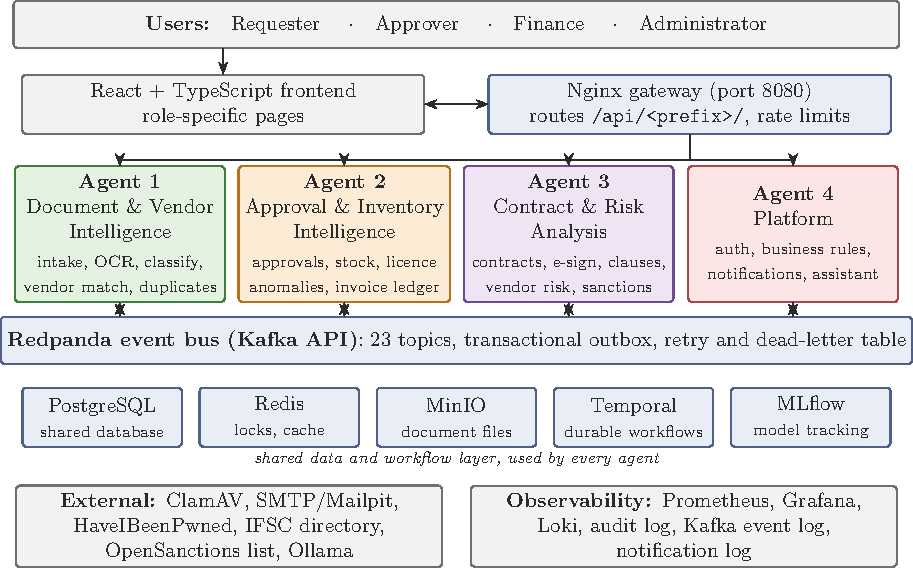
\includegraphics{figures/diagrams/arch}
\caption{Overall architecture of the proposed system}\label{fig:arch}
\end{figure}

This decomposition isolates concerns: a change to extraction does not touch the approval engine, and a slow parse cannot block an upload, because heavy work runs in background workers off the request path.

\subsection{The Four Agents}
Table~\ref{tab:agents} summarises the agents, and the paragraphs that follow describe what each one does. In the sense defined in Section~\ref{sec:agentdef}, each agent observes events, decides within the limits set by the business rules, acts, and defers to a person when its confidence is low or the action is sensitive.

\begin{table}[!htbp]
\centering\tablestyle
\caption{Summary of the four agents in the proposed system}\label{tab:agents}
\begin{tabularx}{\textwidth}{|L{0.17\textwidth}|L{0.11\textwidth}|L{0.30\textwidth}|Y|}
\hline
\textbf{Agent} & \textbf{Port} & \textbf{Main responsibility} & \textbf{Key techniques} \\ \hline
Document and Vendor Intelligence & 8001 (+ worker) & Document intake, reading, classification, field extraction, vendor matching and onboarding, duplicate detection, bank-detail control & ClamAV, pdfplumber, Docling, PaddleOCR, TF-IDF + logistic regression, LayoutLMv3, rapidfuzz \\ \hline
Approval and Inventory Intelligence & 8002 (+ worker) & Approval routing and authority, SLA escalation, inventory reservation and reorder, licence anomalies and reclaim, invoice ledger & Temporal, Redis locks, Isolation Forest, SHAP \\ \hline
Contract and Risk Analysis & 8003 (+ worker) & Contract generation and signing, clause extraction, renewal reminders, vendor risk scorecard and clearance, sanctions screening, offboarding & Jinja2, Legal-BERT (CUAD), deterministic ruleset engine \\ \hline
Platform & 8004, 8005, chatbot & Authentication and roles, business-rules engine, notifications, conversational assistant & JWT, argon2id, Jinja2, SMTP, Ollama (Llama 3.2 3B) \\ \hline
\end{tabularx}
\end{table}

\paragraph{Document and Vendor Intelligence.} This agent is the entry point for every document, whether uploaded, e-mailed to an intake address or dropped into a watched folder. It checks the file's size and real type, streams it through ClamAV and rejects it if the scanner flags it or cannot be reached, stores it in MinIO and publishes \code{document.ingested} in the same database transaction. A background worker reads, classifies and extracts the document, gives every field a confidence score and sends doubtful results to a review queue. Each invoice is also checked for GST: the supplier's GSTIN, the split between central, state and integrated tax, the rate expected for each HSN or SAC code, the totals and, where present, the signed e-invoice QR code; a failed check forces review but never changes the confidence score. The agent matches the vendor against existing records, books invoices against their purchase request, flags likely duplicates, and never applies new bank details directly: they wait as a pending change until a different user with the finance or admin role verifies them, and payment is held meanwhile.

\paragraph{Approval and Inventory Intelligence.} This agent derives each request's approval chain from spend tiers held in the business-rules engine (automatic up to \Rs 500, a department manager up to \Rs 5,000, and a manager plus the finance head above that) and from an approval-authority matrix that also enforces separation of duties: nobody, including an administrator, can approve their own request. A Temporal workflow per request waits for the decision, reminds the approver at 50\% and 80\% of the SLA and escalates after 48 hours. Stock is reserved under a short Redis lock so that two concurrent requests cannot take the last unit, and a request for an item that is out of stock is created as back-ordered. An Isolation Forest scores licence usage; a licence above the anomaly threshold receives a reclaim request that waits through a seven-day grace period before it reaches an approver. When \code{contract.signed} arrives, the request moves to \emph{ordered}; deliveries are then recorded per line, with asset tags for hardware (\emph{partially received} until everything has arrived, then \emph{fulfilled}), and invoices are matched line by line against the order, with a 1\% tolerance on the unit price and on the order's remaining balance before an invoice is held; once deliveries are recorded, an invoice may not exceed the quantity received. When an invoice is booked, the TDS to deduct is computed from the vendor's or the category's section and threshold. Each new request is also checked against its department's budget for the category and fiscal quarter, and the agent maintains the IT catalog and request-for-quotation events (Section~\ref{sec:extensions}).

\paragraph{Contract and Risk Analysis.} When a request is approved, this agent fills one of three Jinja2 templates (hardware purchase, SaaS subscription or professional services), renders the contract as text and PDF, and sends it for signature automatically. Signing happens in the application: an authorised approver, finance or admin user types or draws a signature, gives consent, and the contract and signer details are sealed with a SHA-256 hash recorded in the audit log and shown on a signature certificate. If the vendor is rated High or has not been scored, the signer must explicitly acknowledge the risk. An HMAC-verified, replay-protected webhook accepts signatures from external providers and is used by the tests. A Legal-BERT model reads the renewal term, notice period and expiration date from the contract text, and a Temporal workflow sends renewal reminders 60, 30 and 15 days before the notice deadline. After signature it reads the obligations the contract contains (Section~\ref{sec:extensions}). The agent also scores each vendor's risk with a deterministic 100-point scorecard, answers whether a vendor is cleared for activation, a purchase or a contract (taking human decisions such as an accepted risk into account), keeps a performance scorecard per vendor, screens vendor names against a sanctions list and news results for adverse media, and handles vendor offboarding by flagging active contracts for review instead of closing them. Every risk score stores its inputs and a SHA-256 hash, so it can be replayed exactly; evidence and disputes from vendors or staff are kept with the score.

\paragraph{Platform.} The fourth agent owns what no functional agent should. The authentication service issues 15-minute JWT access tokens and refresh tokens held in an httpOnly cookie (revoked on logout), hashes passwords with argon2id, verifies e-mail addresses, locks an account after repeated failures and rejects passwords found in known breaches. It also hosts the business-rules engine: 71 rules, such as spend tiers, thresholds and tolerances, that an administrator edits at run time and that services refresh when \code{business_rule.updated} is published. The notification service consumes 17 event topics, sends urgent messages immediately and batches routine ones into digests, retries failed deliveries and logs every message. Finally, a conversational assistant answers questions by retrieval-augmented generation with a local Llama~3.2 (3B) model through Ollama. An index of contract clauses, document text, business rules and current records (requests, vendors, licences, budgets) is embedded with \code{nomic-embed-text} into PostgreSQL with pgvector and kept current every minute; for each question the closest passages the user is allowed to see are retrieved and the model answers only from them, citing their source, and says so when they do not contain the answer. Access is applied when retrieving (staff see everything; a requester only their own requests, contracts and documents), and bank details are masked before indexing.

\subsection{Extensions after the Competitive Analysis}\label{sec:extensions}
The comparison with commercial suites (Section~\ref{sec:commercial}) identified capabilities that matter for IT procurement and that the platform lacked. Five were added without changing the existing flow: each is switched off or advisory by default, uses the existing agents, events and business rules, and is described in Table~\ref{tab:extensions}.

{\tablestyle
\begin{longtable}{|L{0.17\textwidth}|L{0.47\textwidth}|L{0.26\textwidth}|}
\caption{Extensions added after the competitive analysis}\label{tab:extensions}\\
\hline
\textbf{Extension} & \textbf{Behaviour} & \textbf{Agent and rules} \\ \hline
\endfirsthead
\multicolumn{3}{l}{\small\textit{Table \thetable\ (continued)}}\\ \hline
\textbf{Extension} & \textbf{Behaviour} & \textbf{Agent and rules} \\ \hline
\endhead
Budget control & A budget is set per department, IT category (hardware, software, SaaS, services) and fiscal quarter. Its usage is computed from the requests that refer to it---pending, committed after approval, consumed once invoiced---so rejections and cancellations release money without bookkeeping. The budget row is locked while a request is checked, so two concurrent requests cannot both use the last amount. A request that would exceed the budget gets a finance approval step. & Approval and Inventory; seven \code{budget.*} rules \\ \hline
Contract obligations & After signature the contract is read for eleven obligation types: SLA uptime and service credits, licence limits, price-increase cap, audit rights, warranty, termination for convenience, minimum commitment, exit terms, data protection, liability cap and insurance. Each finding waits for a person to confirm it; confirmed obligations get a due date and reminders. Recording a month's measured uptime computes the service credit, and invoices for the request carry a note until the credit is applied. A licence with more users than the contract allows is marked as breached, and licence reclaims respect a minimum commitment. & Contract and Risk;\newline \code{contract.obligation_*},\newline \code{contract.sla_credit_}\newline\code{auto_expect} \\ \hline
IT catalog & Approved items with an agreed price, vendor, lead time, warranty and expiry date. A catalog line takes its price, vendor and request type from the catalog, not from the client; an expired item cannot be ordered. A seat add-on increases the licence's seat count when it is received. Catalog-only requests up to a set amount can skip the manager step. & Approval and Inventory;\newline \code{catalog.preapproved_}\newline\code{max_inr} \\ \hline
Sourcing events (RFQ) & A buyer invites two or more vendors to quote by a deadline. A quote that carries the RFQ reference is linked automatically when the document pipeline reads it. While an RFQ is sealed, no role sees amounts before the deadline. Quotes are scored per criterion---price, lead time, warranty, support, vendor risk band and on-time delivery---and weighted; a shortlist can go to a second round, and the award creates the purchase request. Requests above a threshold without an RFQ or catalog price are flagged. & Approval and Inventory; \code{sourcing.*} \\ \hline
Partial receipts and scorecards & Deliveries are recorded per line with asset tags; an invoice for more than has been received is a variance, completing the three-way match. A scorecard per vendor reports on-time delivery, invoice accuracy, RFQ response rate and SLA breaches, and feeds the RFQ comparison. & Approval and Inventory\newline (\code{invoice.match_}\newline\code{against_received});\newline Contract and Risk \\ \hline
GST and TDS & Every invoice is checked for GST: supplier GSTIN, central and state tax or integrated tax depending on the place of supply, the rate for each HSN or SAC code, and taxable value plus tax equal to the total; reverse charge applies to services from suppliers outside India. An e-invoice QR code is verified against the tax portal's public key and compared with the printed invoice. A failed check forces review and publishes \code{invoice.tax_flagged}, without changing the confidence score. TDS is computed when an invoice is booked, the GSTR-2B statement from the GST portal is reconciled with the books, and payment deadlines for micro and small enterprises are tracked. The rates are seeded values that a chartered accountant must confirm. & Document and Vendor; Approval and Inventory;\newline \code{gst.*}, \code{tds.*}, \code{msme.*} \\ \hline
\end{longtable}}

\subsection{Document Processing Pipeline}
The document pipeline turns an uploaded file into a structured, confidence-scored record (Figure~\ref{fig:pipeline}). The upload returns as soon as the file is stored; a worker processes it in the background.

\begin{figure}[!htbp]
\centering
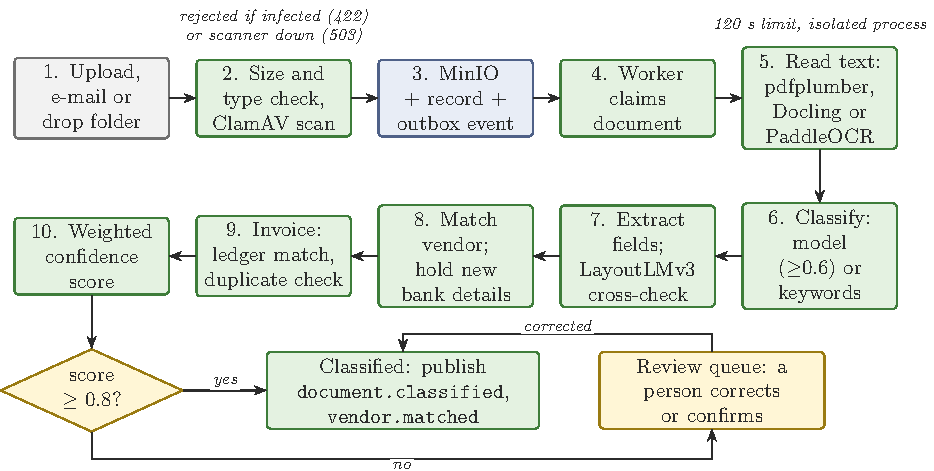
\includegraphics{figures/diagrams/pipeline}
\caption{Document processing pipeline of the Document and Vendor Intelligence agent}\label{fig:pipeline}
\end{figure}

A file is rejected before storage if it is empty, too large (25\,MB at the gateway), of a type that its bytes do not confirm, infected, or if ClamAV cannot be reached, so the intake fails closed. After the file and its database row are stored, the worker reads it in a separate process with a 120-second limit: pdfplumber for PDFs with a usable text layer, Docling for scanned PDFs, and PaddleOCR for images after deskewing and upscaling by at most 1.5 times. The classifier labels the document as an invoice, purchase order, quotation or other paperwork, and regular expressions extract the vendor name, document number, date, currency, totals and line items. When LayoutLMv3 is installed it reads the document independently, and a disagreement forces review. The vendor name is normalised and matched against existing vendors with a fuzzy ratio of at least 88, or a new vendor record is created; first-seen bank details are held for verification. An invoice is booked against its purchase request and checked for duplicates: same vendor, an amount within 2\%, a date within 7 days and a document number at least 85\% similar (all three values are business rules). Finally, the per-field confidence scores are combined into an overall score (Section~\ref{sec:code}); a document scoring below 0.8 goes to the review queue, and reviewers' corrections are kept as per-vendor hints for later documents. Any dependency failure returns the document to the queue to be retried, up to five attempts.

\subsection{Inter-Agent Communication and Workflow}
Every event uses the same envelope (event ID, event type, timestamp, source service, correlation ID and payload), and the 23 topics and their payloads are fixed in a shared contract document so that producers and consumers could be built in parallel. Each service authenticates to the broker with its own SASL/SCRAM account and may use only its own topics. Events are written to an outbox table in the same transaction as the change that caused them and relayed to the broker afterwards; consumers are idempotent, retry failures and move events that keep failing to a dead-letter table shown on the Control Panel. Figure~\ref{fig:events} shows the main flows and Table~\ref{tab:events} lists the topics.

\begin{figure}[!htbp]
\centering
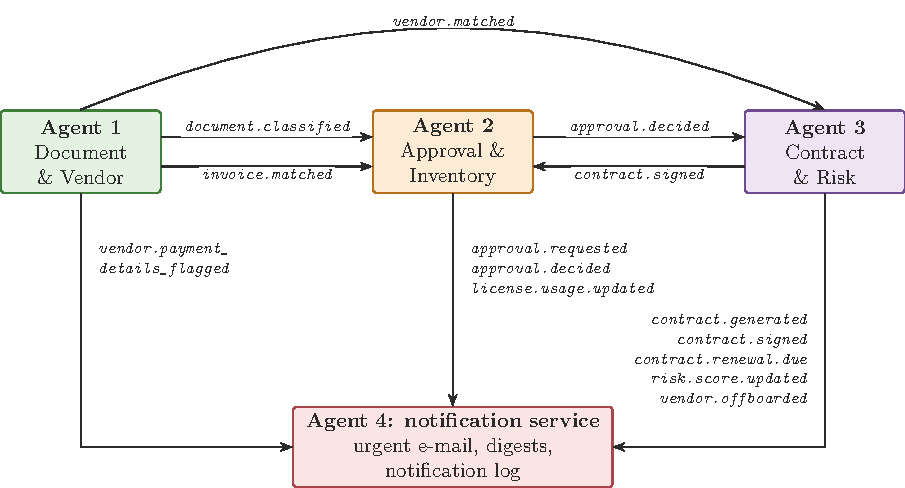
\includegraphics{figures/diagrams/events}
\caption[Main event flows between the agents]{Main event flows between the agents. Rule changes (\code{business_rule.updated}) are broadcast to every agent and are omitted for clarity.}\label{fig:events}
\end{figure}

\begin{longtable}{|L{0.36\textwidth}|L{0.13\textwidth}|L{0.41\textwidth}|}
\caption{Event topics exchanged between the agents}\label{tab:events}\\
\hline
\textbf{Topic} & \textbf{Published by} & \textbf{Consumed by and purpose} \\ \hline
\endfirsthead
\multicolumn{3}{l}{\small\textit{Table \thetable\ (continued)}}\\ \hline
\textbf{Topic} & \textbf{Published by} & \textbf{Consumed by and purpose} \\ \hline
\endhead
\code{document.ingested} & Agent 1 & Agent 1 worker: starts the pipeline \\ \hline
\code{document.classified} & Agent 1 & Agent 2: turns a quote into a purchase request; notifications \\ \hline
\code{vendor.matched} & Agent 1 & Agent 3: scores the vendor's risk \\ \hline
\code{vendor.payment_}\newline\code{details_flagged} & Agent 1 & Notifications: urgent alert on a pending bank-detail change \\ \hline
\code{invoice.matched} & Agent 1 & Agent 2: updates the invoice ledger and request status \\ \hline
\code{approval.requested} & Agent 2 & Notifications: tells the approver \\ \hline
\code{approval.decided} & Agent 2 & Agent 3: generates the contract; Agent 1: books invoices waiting for the request; notifications \\ \hline
\code{license.usage.updated} & Agent 2 & Notifications: utilisation and anomaly alerts \\ \hline
\code{order.summary.generated} & Agent 2 & Control Panel: hourly open-order summary \\ \hline
\code{contract.generated} & Agent 3 & Notifications \\ \hline
\code{contract.signed} & Agent 3 & Agent 2: request becomes \emph{ordered}; notifications \\ \hline
\code{contract.renewal.due} & Agent 3 & Notifications: 60, 30 and 15-day reminders (urgent at 15) \\ \hline
\code{risk.score.updated} & Agent 3 & Notifications: urgent for the High band \\ \hline
\code{vendor.offboarded} & Agent 3 & Notifications: offboarding summary and contracts flagged \\ \hline
\code{reminder.due} & Agents 1--3 & Notifications: reminder to whoever must act; Control Panel \\ \hline
\code{business_rule.updated} & Agent 4 & Agents 1--3: refresh their cached rules \\ \hline
\code{notification.send} & Any service & Notifications: generic message \\ \hline
\code{budget.threshold_crossed} & Agent 2 & Notifications: budget warning or overrun \\ \hline
\code{rfq.issued} & Agent 2 & Notifications: invitation to each invited vendor \\ \hline
\code{rfq.awarded} & Agent 2 & Notifications: award and thank-you messages \\ \hline
\code{goods.received} & Agent 2 & Notifications: delivery recorded \\ \hline
\code{contract.obligation.due} & Agent 3 & Notifications: obligation due, overdue or breached \\ \hline
\code{invoice.tax_flagged} & Agent 1 & Control Panel: failed GST check \\ \hline
\end{longtable}

In a typical run, a requester creates a purchase request, or a vendor quote is dropped into the intake folder and Agent~1 classifies it and Agent~2 creates the request from it. Agent~2 builds the approval chain and, once the last approver agrees, publishes \code{approval.decided}. Agent~3 generates the contract and sends it for signature, and its \code{contract.signed} event moves the request to \emph{ordered}. The notification service follows all of these events, sending urgent alerts such as an approval request or a flagged bank-detail change immediately and batching routine ones into a digest. Every API request receives a correlation ID at the gateway, which is carried through the events and log lines of every service, so the whole journey of one request can be followed in Grafana.

\subsection{Use Case View}
Figure~\ref{fig:usecase} presents the use cases of the four roles. The \emph{Requester} raises purchase requests, uploads documents and follows their progress; the \emph{Approver} decides the requests and licence reclaims assigned to them in the approval-authority matrix and can sign contracts; the \emph{Finance} user verifies bank-detail changes, onboards vendors, maintains risk signals and can also approve and sign; and the \emph{Administrator} manages users and business rules, monitors the system and offboards vendors. Administrators can perform every action, so the diagram shows each role only with the actions specific to it.

\begin{figure}[!htbp]
\centering
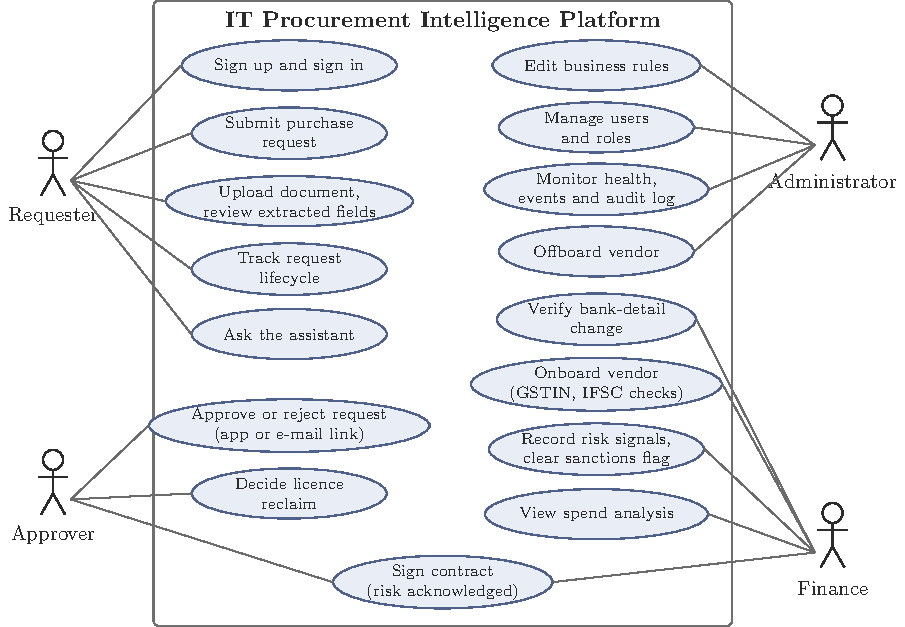
\includegraphics{figures/diagrams/usecase}
\caption{Use case diagram of the IT procurement platform}\label{fig:usecase}
\end{figure}

The use cases group into five phases:
\begin{enumerate}
  \item \textbf{Authentication and business rules.} Users sign up, verify their e-mail and sign in; an administrator assigns roles and edits the business rules (spend tiers, SLA, thresholds and tolerances) on the Business Rules page, with every change kept in a history.
  \item \textbf{Purchase and inventory.} A requester submits a purchase request, stock is checked and reserved, the approval workflow runs in Temporal, and the approver approves or rejects.
  \item \textbf{Vendor intelligence.} Vendor documents are read and matched, new vendors are onboarded with identifier checks, bank details are verified by a second person, and a vendor risk score is calculated.
  \item \textbf{Contract and risk.} A contract is generated for the approved request, sent for signature, signed in the application after the vendor's risk is shown, and renewal reminders are scheduled.
  \item \textbf{Notification.} Approvals, flagged bank details, renewals, risk changes and signatures trigger e-mail notifications to the people concerned.
\end{enumerate}

\subsection{Key Design Principles}
Four principles run through the design. The system is \emph{fraud-aware}: uploads are scanned and rejected if the scanner is unavailable, bank details need a second person's verification, the webhook is accepted only with a valid HMAC signature and never twice, and signing a contract with a High-risk vendor requires an explicit acknowledgement. It is \emph{human-centred}: results below the confidence threshold go to review, a licence reclaim waits for the holder and an approver, offboarding flags contracts rather than closing them, and the models never retrain themselves. It is \emph{accountable}: significant actions are written to an audit log, identity is always taken from the JWT and never from a request body, business-rule changes are versioned, and every model-routing decision is logged. Finally, it is \emph{observable}: every service exposes Prometheus metrics, logs carry a correlation ID, the Control Panel shows every Kafka event and every failed event, and a System Health page shows the state of the services.

\subsection{Technology Stack}
Table~\ref{tab:stack} lists the main technologies. Pretrained open-source components are used wherever possible; the models trained within the project are the document classifier, the licence-anomaly model and the vendor risk model.

\begin{table}[!htbp]
\centering\tablestyle
\caption{Technology stack of the proposed system}\label{tab:stack}
\begin{tabularx}{\textwidth}{|L{0.18\textwidth}|L{0.38\textwidth}|Y|}
\hline
\textbf{Layer} & \textbf{Technology} & \textbf{Purpose} \\ \hline
Frontend & React, TypeScript, Vite, Tailwind CSS & Role-based pages, one home page per item \\ \hline
Gateway & Nginx & Single entry point; routes \texttt{/api/<prefix>/}, rate limits, security headers \\ \hline
Backend services & FastAPI (Python), SQLAlchemy, Alembic, Docker Compose & One containerised service per agent, plus workers \\ \hline
Messaging & Redpanda (Kafka API), aiokafka, SASL/SCRAM & Events between agents, per-service topic permissions \\ \hline
Workflow engine & Temporal & Approval SLAs, reclaim grace period, renewal reminders \\ \hline
Data stores & PostgreSQL, Redis, MinIO & Records, locks and caches, document files \\ \hline
Document AI & pdfplumber, Docling, PaddleOCR, LayoutLMv3, rapidfuzz & Text extraction, OCR, cross-check, vendor and duplicate matching \\ \hline
Models & scikit-learn (logistic regression, Isolation Forest)~\cite{pedregosa2011sklearn}, SHAP, Legal-BERT (Hugging Face Transformers), MLflow & Classification, licence anomalies, clause extraction, experiment tracking (vendor risk uses a deterministic ruleset) \\ \hline
Assistant & Ollama (Llama 3.2 3B, nomic-embed-text), PostgreSQL pgvector & Retrieval-augmented answers from contracts, documents, rules and current records, with citations \\ \hline
Security & JWT, argon2id~\cite{biryukov2016argon2}, HMAC-SHA256, ClamAV, HaveIBeenPwned & Authentication, password hashing, webhook verification, malware scanning, breached-password check \\ \hline
Monitoring & Prometheus, Grafana, Loki, Promtail, kafka-exporter & Metrics, dashboards, centralised logs by correlation ID, consumer lag \\ \hline
Notifications & Jinja2 templates, SMTP (Mailpit in development) & Templated e-mail \\ \hline
\end{tabularx}
\end{table}

% Chapter 4: Design of the System

\chapter{Design of the System} \label{chap4}
\newpage

This chapter describes the requirements, development approach, system models, resource requirements and architecture of the platform. It presents the functional and non-functional requirements, the data flows, the main UML views, the database design and the system layers.

\section{Requirement Engineering}
Requirement engineering identifies the capabilities expected from the platform and keeps them consistent during development. It is central here because the system is divided into services that must interoperate through shared event formats, database tables, REST conventions and authentication rules.

\subsection{Requirement Elicitation}
Requirements were identified from the following sources:
\begin{itemize}
  \item \textbf{Existing practices and literature:} the review in Chapter~\ref{chap2} and the problem analysis in Chapter~\ref{chap3} identified the recurring problems: repeated manual data entry, unverified vendor details, duplicate invoices, delayed approvals, under-used licences, missed renewals and infrequent vendor-risk reviews.
  \item \textbf{Stakeholder analysis:} the users are requesters, approvers, finance users and system administrators, implemented as the four roles \emph{requester}, \emph{approver}, \emph{finance} and \emph{admin}.
  \item \textbf{Guide and mentor reviews:} reviews with the guides prioritised features and separated what could be built from what depends on paid accounts; the changes requested in a mentor review on 29 August 2026 were tracked to completion.
  \item \textbf{Review of tools and datasets:} document-processing tools, workflow engines and public datasets were tried against their expected inputs and practical limits. For example, PaddleOCR's native engine crashed the worker process on some platform and version combinations, which led to running it in an isolated subprocess rather than dropping it; and the CUAD dataset was chosen to evaluate clause extraction.
\end{itemize}
The requirements were then grouped into functional and non-functional requirements.

\subsection{Software Lifecycle Model}
The project followed an iterative and incremental model (Figure~\ref{fig:sdlc}). This suited a system whose thresholds, approval rules, models and integration details had to be tested and refined during implementation. Each team member owned one service. The main practices were:
\begin{itemize}
  \item \textbf{Contract-first design:} the Kafka event envelope and topic payloads, the base database schema, the REST response envelope and the authentication middleware were agreed before the services were built in parallel.
  \item \textbf{Service-wise increments:} the work was divided across the document and vendor, approval and inventory, contract and risk, and notification and authentication services.
  \item \textbf{Integration iterations:} the services were connected behind one gateway. Integration exposed problems in gateway routing, broker addressing, UUID column types and colliding migration tables, which were fixed at the shared level.
  \item \textbf{Continuous testing and audits:} unit and end-to-end tests were written alongside the features, and two quality audits re-tested the running system, with a regression test added for each defect fixed.
  \item \textbf{Repeatable deployment:} a single \code{run.sh} script builds and starts the whole containerised stack from a clean clone.
\end{itemize}

\begin{figure}[!htbp]
\centering
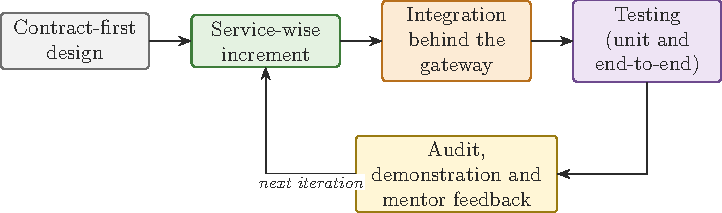
\includegraphics{figures/diagrams/sdlc}
\caption{Iterative and incremental development cycle}\label{fig:sdlc}
\end{figure}

\subsection{Requirement Analysis}
The requirements are grouped into functional requirements, which describe what the system does, and non-functional requirements, which describe the qualities and constraints it must satisfy. Every threshold mentioned below is a business rule that an administrator can change at run time; the values given are the current settings.

\subsubsection{Functional Requirements}
Table~\ref{tab:fr} lists the functional requirements and the agent responsible for each.

{\tablestyle
\begin{longtable}{|L{0.07\textwidth}|L{0.64\textwidth}|L{0.17\textwidth}|}
\caption{Functional requirements}\label{tab:fr}\\
\hline
\textbf{ID} & \textbf{Requirement} & \textbf{Agent} \\ \hline
\endfirsthead
\multicolumn{3}{l}{\small\textit{Table \thetable\ (continued)}}\\ \hline
\textbf{ID} & \textbf{Requirement} & \textbf{Agent} \\ \hline
\endhead
FR1 & Users can sign up, confirm their e-mail address, sign in and receive a 15-minute access token and a refresh token that logout revokes. Every endpoint checks the token and the role, except the health and metrics endpoints and the HMAC-authenticated signature webhooks. & Platform \\ \hline
FR2 & An administrator can view and edit the business rules (spend tiers, SLA, thresholds and tolerances); each change is versioned and reaches every service without a restart. & Platform \\ \hline
FR3 & Documents can be uploaded, e-mailed to an intake address or dropped into a watched folder. Each file is size- and type-checked and scanned for malware before storage; it is rejected if the scanner is unavailable. & Document and Vendor \\ \hline
FR4 & Documents are classified as invoice, purchase order, quotation or other; vendor, document number, date, currency, totals and line items are extracted. & Document and Vendor \\ \hline
FR5 & Each extracted field receives a confidence score. Documents below the threshold (0.8) go to a review queue, where fields can be corrected or confirmed. & Document and Vendor \\ \hline
FR6 & Vendors are matched by normalised name (fuzzy threshold 88); onboarding validates GSTIN format and check digit and IFSC codes and flags possible impostors. & Document and Vendor \\ \hline
FR7 & New or changed bank details stay pending, with payment held, until verified by a different user with the finance or admin role. & Document and Vendor \\ \hline
FR8 & Likely duplicate invoices are flagged (same vendor, amount within 2\%, date within 7 days, document number at least 85\% similar). & Document and Vendor \\ \hline
FR9 & Purchase requests follow approval chains by spend tier (automatic up to \Rs 500, manager up to \Rs 5,000, manager and finance above) and an approval-authority matrix; nobody can approve their own request. & Approval and Inventory \\ \hline
FR10 & Each request's approval runs as a durable Temporal workflow with reminders at 50\% and 80\% of the SLA; after 48 hours the request escalates to the next approver, and a timeout at the last level rejects it. Approvers can also decide from a single-use e-mail link for amounts up to \Rs 50,000. & Approval and Inventory \\ \hline
FR11 & Stock is reserved under a Redis lock so that concurrent requests cannot reserve the same unit; a request for out-of-stock items is back-ordered, and reorder suggestions are computed. & Approval and Inventory \\ \hline
FR12 & Licence usage is scored by an anomaly-detection model with per-licence explanations; an anomalous licence receives a reclaim request that waits through a seven-day grace period before approval. & Approval and Inventory \\ \hline
FR13 & Invoices are matched line by line against the purchase request, and an invoice exceeding the price or remaining balance by more than 1\% is held. & Approval and Inventory \\ \hline
FR14 & Contracts are generated from templates after approval and sent for signature automatically; renewal type, notice period and end date are extracted, and reminders are scheduled 60, 30 and 15 days before the notice deadline. & Contract and Risk \\ \hline
FR15 & Contracts are signed in the application with consent and a sealed audit record; signing for a vendor that is not cleared (High, provisional or unscored) requires an acknowledgement. External signature callbacks are accepted only with a valid HMAC signature and only once. & Contract and Risk \\ \hline
FR16 & Vendor risk is an integer score out of 100 from a deterministic ruleset, with a Low, Medium or High band and a rating status (assessed, provisional or not rated); a vendor with incomplete checks is never shown as Low, and a cancelled GSTIN, an invalid bank route or a potential sanctions match forces High until it is resolved. & Contract and Risk \\ \hline
FR17 & A clearance check states whether a vendor may be used for activation, a purchase or a contract; post-score decisions (approve, approve with conditions, accept risk, reject), evidence and disputes are recorded, and every score can be replayed exactly. & Contract and Risk \\ \hline
FR18 & Vendor offboarding revokes the vendor's access, flags active contracts for review and sets a data-retention flag instead of deleting records. & Contract and Risk \\ \hline
FR19 & The notification service consumes events, sends templated e-mail, sends urgent items immediately and batches routine ones into digests, retries failures and keeps a searchable log. & Platform \\ \hline
FR20 & An assistant answers questions from the platform's own contracts, documents, rules and records by retrieval-augmented generation, cites its sources, says when it cannot find an answer, and retrieves only what the asking user may see. & Platform \\ \hline
FR21 & The frontend provides role-specific navigation and dashboards, a request wizard, an approval inbox, one home page per request, document, vendor, licence and contract, and pages for notifications, spend analysis, business rules, users, audit activity, system health and the Kafka event log. & Frontend \\ \hline
FR22 & Significant actions on documents, vendors, requests and contracts are written to an audit log that administrators can query. & All \\ \hline
FR23 & Each request is checked against its department's budget for the category and fiscal quarter; a request that would exceed it receives a finance approval step, and concurrent requests cannot both use the last amount. & Approval and Inventory \\ \hline
FR24 & Obligations are read from signed contracts and confirmed by finance; confirmed obligations are reminded before their due date, recorded downtime yields the contractual service credit, and a licence with more users than the contract allows is flagged. & Contract and Risk \\ \hline
FR25 & Requesters order from an IT catalog whose agreed prices, vendor and type override client input; expired items cannot be ordered, and a received seat add-on increases the licence's seats. & Approval and Inventory \\ \hline
FR26 & Finance runs request-for-quotation events with sealed quotes, quotes linked from the document pipeline by reference, weighted comparison, further rounds and an award that creates the purchase request. & Approval and Inventory \\ \hline
FR27 & Deliveries are recorded per line with asset tags; invoices may not exceed the quantity received; each vendor has a performance scorecard. & Approval and Inventory, Contract and Risk \\ \hline
FR28 & Every invoice is checked for GST (GSTIN, tax split, rate per HSN or SAC code, totals, e-invoice QR signature); a failed check forces review without changing the confidence score. TDS is computed at booking, the GSTR-2B statement is reconciled, and MSME payment deadlines are tracked. & Document and Vendor, Approval and Inventory \\ \hline
\end{longtable}}

\subsubsection{Non-Functional Requirements}
Table~\ref{tab:nfr} lists the qualities and constraints the system must satisfy.

\begin{table}[!htbp]
\centering\tablestyle
\caption{Non-functional requirements}\label{tab:nfr}
\begin{tabularx}{\textwidth}{|L{0.18\textwidth}|Y|}
\hline
\textbf{Category} & \textbf{Requirement} \\ \hline
Security & JWT authentication and role checks in every service; identity taken only from the token; argon2id password hashing and breached-password check; account lockout and gateway rate limits; fail-closed malware scanning; HMAC-verified webhooks; dual control of payment details; per-service Kafka credentials and topic permissions; only the gateway port exposed. \\ \hline
Reliability & Approval, reclaim and renewal workflows are durable (Temporal). Events are published through a transactional outbox; consumers are idempotent, retry and dead-letter failures; a sweep re-queues stranded documents; a timed-out last approval is rejected, never approved by default. \\ \hline
Consistency & A common REST envelope and error format; a purchase-request state machine enforced in code and by a database constraint; idempotent migrations owned by each service. \\ \hline
Performance & Uploads return once the file is stored; reading, OCR and model inference run in background workers with time limits. \\ \hline
Traceability & Every event carries an event ID, source and correlation ID; logs from every service are collected centrally and searchable by correlation ID; significant actions are audited; model-routing decisions are logged. \\ \hline
Explainability & Confidence scores per field, risk factors per vendor, SHAP reasons per licence and the risk shown before signing. \\ \hline
Maintainability & Responsibilities separated by service; shared contracts documented; thresholds held as business rules, each with a behaviour test. \\ \hline
Portability & The stack is containerised and runs on macOS, Linux and Windows through WSL2. \\ \hline
\end{tabularx}
\end{table}

\noindent\textbf{Constraints and assumptions.} Payment execution, ERP integration, a third-party e-signature provider and automatic model retraining are outside the scope. GST and TDS rates are seeded values that a chartered accountant must confirm. Kafka traffic is authenticated but not encrypted, which is acceptable only on a single host. The vendor risk data, licence usage logs, classifier corpus and sample documents are synthetic.

\subsection{UML Diagrams and Data Flow Diagrams}

\subsubsection{Use Case Diagram}
The use case diagram is shown in Figure~\ref{fig:usecase} in Chapter~\ref{chap3}. It identifies the Requester, Approver, Finance user and Administrator and groups their activities into authentication and rules, purchase and inventory, vendor intelligence, contract and risk, and notification.

\subsubsection{Data Flow Diagram -- Level 0}
The context diagram (Figure~\ref{fig:dfd0}) shows the platform as a single process and its exchanges with the external entities: the three groups of users, vendors who send documents, the e-mail service, and the external lookup services.

\begin{figure}[!htbp]
\centering
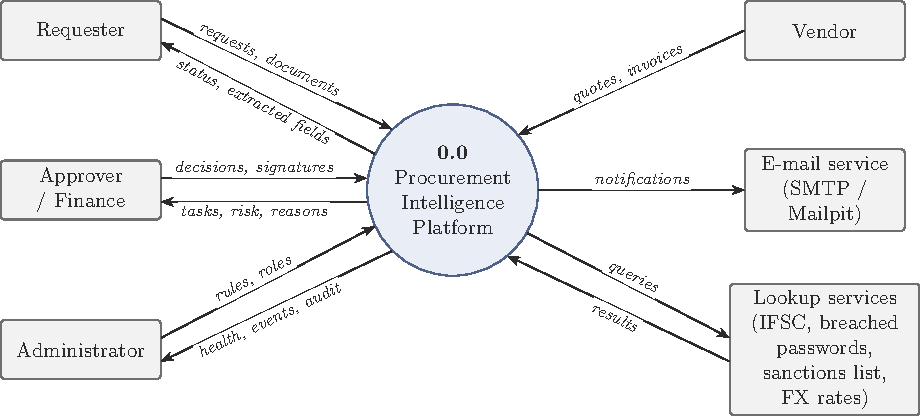
\includegraphics{figures/diagrams/dfd0}
\caption{Level 0 data flow diagram (context diagram)}\label{fig:dfd0}
\end{figure}

\subsubsection{Data Flow Diagram -- Level 1}
The Level 1 diagram (Figure~\ref{fig:dfd1}) decomposes the platform into the processes of Table~\ref{tab:dfd}. Processes 2.0 to 5.0 exchange events through the messaging layer, process 6.0 consumes them, and process 1.0 issues the tokens and rules that the others check.

\begin{figure}[!htbp]
\centering
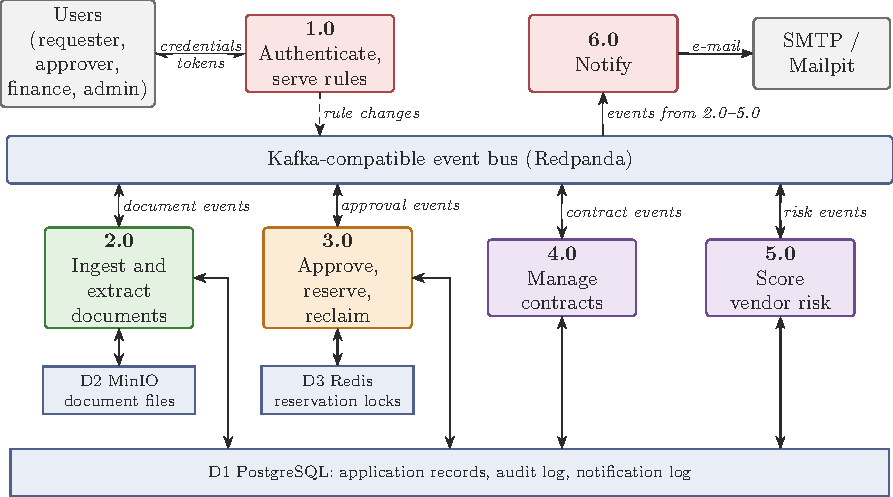
\includegraphics{figures/diagrams/dfd1}
\caption{Level 1 data flow diagram}\label{fig:dfd1}
\end{figure}

\begin{table}[!htbp]
\centering\tablestyle
\caption{Level 1 DFD processes}\label{tab:dfd}
\begin{tabularx}{\textwidth}{|C{0.09\textwidth}|L{0.18\textwidth}|L{0.26\textwidth}|Y|}
\hline
\textbf{Process} & \textbf{Name} & \textbf{Inputs} & \textbf{Outputs} \\ \hline
1.0 & Authenticate, serve rules & Credentials, refresh token, rule edits & Access and refresh tokens, role, rule changes \\ \hline
2.0 & Ingest and extract documents & Uploaded, e-mailed or dropped file & Classified document, vendor match, review-queue items, invoice match \\ \hline
3.0 & Approve, reserve, reclaim & Purchase request, decisions, usage logs & Decisions, reservations, escalations, reclaim requests \\ \hline
4.0 & Manage contracts & Approved request, signature & Contract text and PDF, signature record, renewal reminders \\ \hline
5.0 & Score vendor risk & Vendor signals, sanctions list & Points per check, band, rating status, overrides, clearance \\ \hline
6.0 & Notify & Events from 2.0--5.0 & E-mail, digests, notification log \\ \hline
\end{tabularx}
\end{table}

\subsubsection{Sequence Diagram}
Figure~\ref{fig:sequence} follows one purchase request from creation to signature. It shows the synchronous calls through the gateway, the asynchronous events, and the point at which the Temporal workflow hands the decision back to the service.

\begin{figure}[!htbp]
\centering
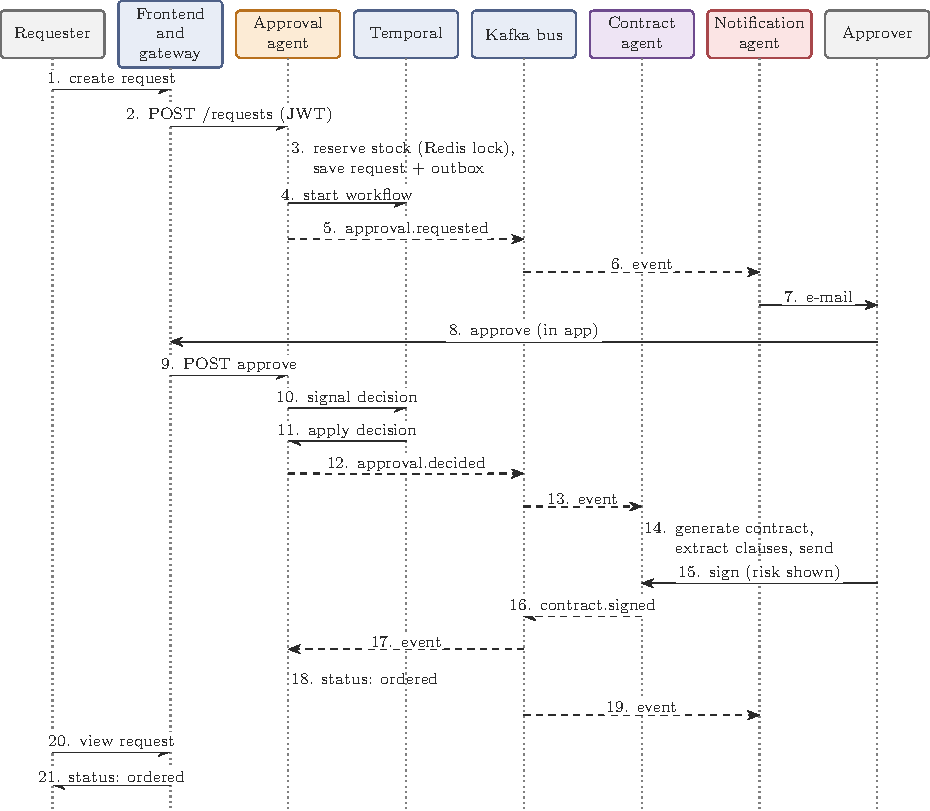
\includegraphics{figures/diagrams/sequence}
\caption[Sequence diagram of the purchase-request journey]{Sequence diagram of the purchase-request journey (solid: synchronous call; dashed: asynchronous event)}\label{fig:sequence}
\end{figure}

\subsubsection{Activity Diagram: Document Processing}
The activity diagram (Figure~\ref{fig:activity}) shows the decisions taken for one document. The upload is rejected if the file fails a check, is infected or cannot be scanned; a file that cannot be read fails with a message for the uploader. A readable file is classified, extracted, matched and scored. A document meeting the threshold, with no rule forcing review, is completed; otherwise it waits in the review queue until a reviewer corrects or confirms it.

\begin{figure}[!htbp]
\centering
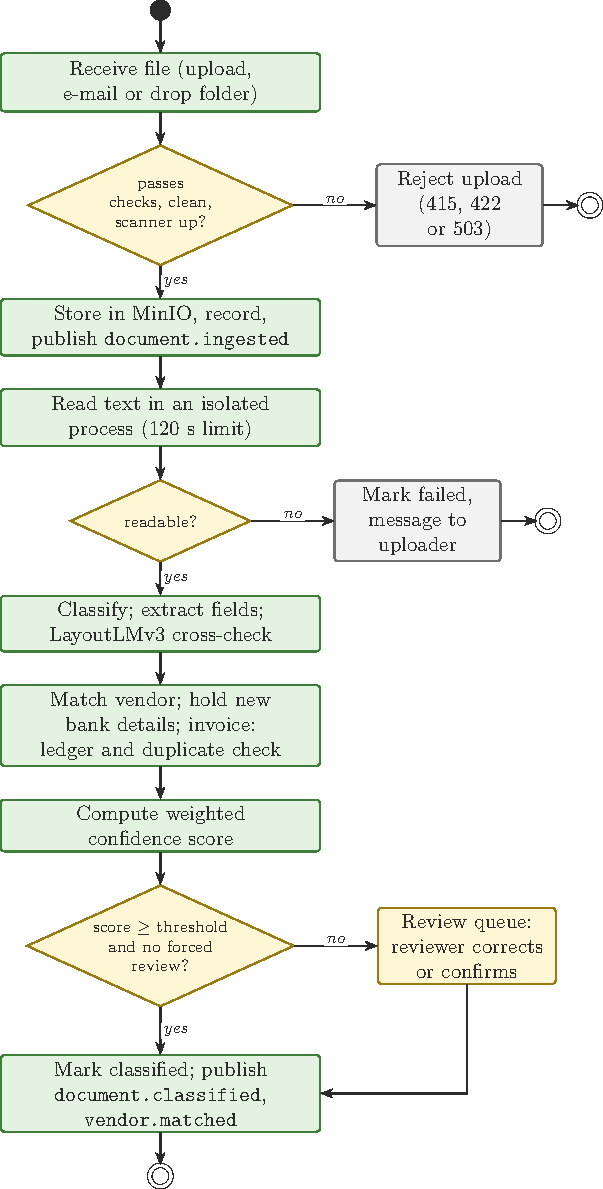
\includegraphics{figures/diagrams/activity}
\caption{Activity diagram of document processing}\label{fig:activity}
\end{figure}

\subsubsection{Purchase-Request State Machine}
A purchase request moves through the states of Figure~\ref{fig:states}. The allowed transitions are defined once in a shared module and checked on every status change, and the database rejects any status outside the list. An event that arrives after the request has already moved past the state it would cause (for example a late \code{contract.signed}) is recognised and ignored rather than treated as an error.

\begin{figure}[!htbp]
\centering
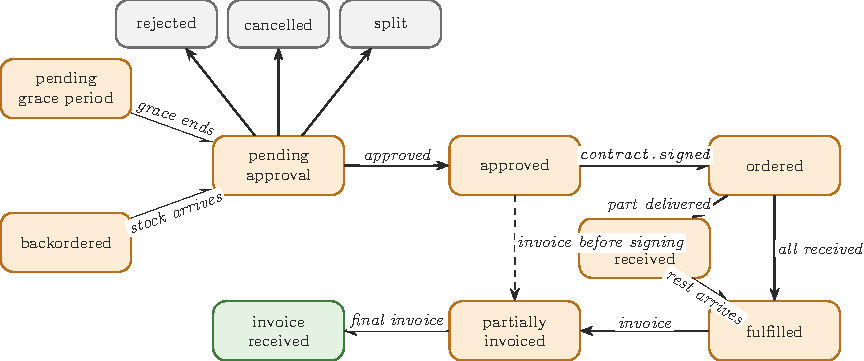
\includegraphics{figures/diagrams/states}
\caption[State machine of a purchase request]{State machine of a purchase request (main transitions; stored state names use underscores, for example \code{pending_approval}; a request can also be cancelled from the waiting states)}\label{fig:states}
\end{figure}

\subsubsection{Entity Relationship Diagram}
All services share one PostgreSQL database of about fifty tables; each service creates and migrates its own. Figure~\ref{fig:er} shows the main entities and their foreign keys as they exist in the running database. The vendor is the central entity: documents, purchase requests, contracts, licences, risk scores, sanctions screenings and payment-change requests all refer to it. The \code{inventory} table has no foreign key: requests refer to stock by SKU inside their items. The extensions of Section~\ref{sec:extensions} add \code{budgets}, \code{contract_obligations}, \code{obligation_events}, \code{sla_credits}, \code{catalog_items}, \code{rfq_events}, \code{rfq_invitations}, \code{rfq_responses}, \code{goods_receipts}, \code{vendor_scorecards}, \code{gst_rates}, \code{gstr2b_uploads} and \code{tds_sections}, and the deterministic risk scorecard adds \code{risk_rulesets}, \code{risk_score_rule_results}, \code{vendor_signal_observations}, \code{vendor_signal_raw_responses}, \code{vendor_evidence}, \code{vendor_assessment_disputes} and \code{vendor_decisions} (scores and observations are append-only); each refers to a request, contract, licence or vendor of the figure. Supporting tables, not shown, hold users and tokens, business rules and their history, the event outbox, inbox and dead-letter table, the Kafka event log, notification and model-routing logs, the reviewer-feedback tables, and the assistant's chat sessions and \code{document_embeddings} index (one row per passage, with its 768-dimensional vector, source, section and audience).

\begin{figure}[!htbp]
\centering
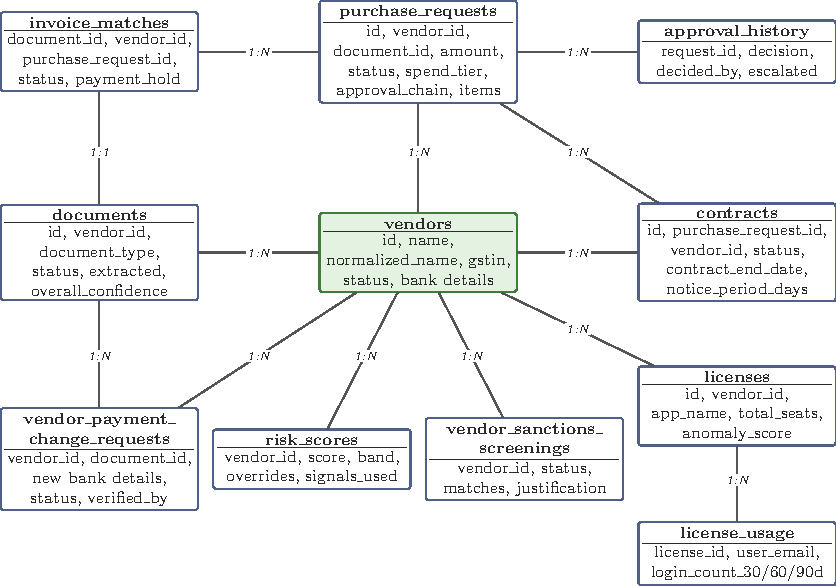
\includegraphics{figures/diagrams/er}
\caption[Entity relationship diagram of the main entities]{Entity relationship diagram of the main entities (foreign keys as in the running database; \code{invoice_matches} also refers to \code{vendors})}\label{fig:er}
\end{figure}

\subsection{Cost Analysis}
The project uses only open-source software and free API tiers, so it incurs no software-licence cost, and it was developed on the team's own laptops. The potential costs are team effort, paid API tiers if live registry lookups are enabled, cloud hosting, and a production e-mail service. The estimates in Table~\ref{tab:cost} are indicative and should be revised against real quotations.

\begin{table}[!htbp]
\centering\tablestyle
\caption{Indicative cost analysis}\label{tab:cost}
\begin{tabularx}{\textwidth}{|L{0.18\textwidth}|Y|L{0.20\textwidth}|}
\hline
\textbf{Item} & \textbf{Basis} & \textbf{Indicative cost} \\ \hline
Software licences & Python, FastAPI, PostgreSQL, Redis, Redpanda, MinIO, Temporal, MLflow, Prometheus, Grafana, Loki, ClamAV, Docling, PaddleOCR, Hugging Face models, Ollama, React and Docker are open source & \Rs 0 \\ \hline
Development hardware & Existing student laptops & \Rs 0 additional \\ \hline
External APIs & HaveIBeenPwned range API, IFSC directory and Frankfurter exchange rates are free; the OpenSanctions list is free for non-commercial use only (CC BY-NC 4.0) and needs a licence for commercial use; live GSTIN lookups depend on the provider's quota & \Rs 0 in the project; depends on usage and licensing in production \\ \hline
Team effort & Part-time project work by four students & Not monetised \\ \hline
Optional cloud hosting & One virtual machine with about 4--8 vCPU and 16\,GB RAM, plus storage and backups & Approx.\ \Rs 6,000--10,000 per month \\ \hline
E-mail delivery & Production SMTP service instead of the development mail catcher & A few hundred rupees per month at pilot volume \\ \hline
\end{tabularx}
\end{table}

A meaningful break-even estimate needs measured document volumes, licence costs and the time saved or duplicate payments avoided. Those figures are not available, so no return-on-investment claim is made.

\subsection{Hardware and Software Requirements}
The stack runs 24 containers on one Docker host. Measured on 16 October 2026, it used about 3.2\,GB of RAM when idle and more while reading scanned documents, and its images occupied about 15\,GB before build cache and data volumes. ClamAV alone needs about 1\,GB of memory. Table~\ref{tab:hw} gives the resulting requirements and Table~\ref{tab:sw} the software.

\begin{table}[!htbp]
\centering\tablestyle
\caption{Hardware requirements}\label{tab:hw}
\begin{tabularx}{\textwidth}{|L{0.16\textwidth}|L{0.34\textwidth}|Y|}
\hline
\textbf{Component} & \textbf{Minimum} & \textbf{Recommended} \\ \hline
Processor & 4 cores & 8 cores \\ \hline
Memory & 8\,GB available to Docker & 16\,GB RAM \\ \hline
Storage & 40\,GB free & 80\,GB free for images, models (about 1\,GB), sanctions data and volumes \\ \hline
Network & Required for the first build, model and sanctions downloads, and sign-up's breached-password check & Broadband connection \\ \hline
GPU & Not required & Optional, for faster OCR and transformer inference \\ \hline
\end{tabularx}
\end{table}

\begin{table}[!htbp]
\centering\tablestyle
\caption{Software requirements}\label{tab:sw}
\begin{tabularx}{\textwidth}{|L{0.20\textwidth}|Y|}
\hline
\textbf{Category} & \textbf{Requirement} \\ \hline
Operating system & macOS, Ubuntu/Linux, or Windows 10/11 with WSL2 \\ \hline
Container runtime & Docker Engine or Docker Desktop with Compose v2 \\ \hline
Backend & Python 3.11, FastAPI, SQLAlchemy, Alembic, pytest, scikit-learn, SHAP, Transformers, rapidfuzz, Jinja2 \\ \hline
Frontend & React, TypeScript, Vite and Tailwind CSS, built in a Node 20 container \\ \hline
Data and messaging & PostgreSQL, Redis, Redpanda (Kafka API) and MinIO \\ \hline
Workflow and ML & Temporal, MLflow \\ \hline
Document processing & pdfplumber, Docling, PaddleOCR, LayoutLMv3 (optional download), ClamAV \\ \hline
Monitoring and mail & Prometheus, Grafana, Loki, Promtail, kafka-exporter, Mailpit \\ \hline
Assistant & Ollama on the host with Llama 3.2 (3B) and nomic-embed-text; PostgreSQL with pgvector \\ \hline
Gateway and browser & Nginx; a current Chrome, Edge, Firefox or Safari \\ \hline
\end{tabularx}
\end{table}

\section{System Architecture}
The platform follows a modular, event-driven architecture in which independent services each own one procurement function. The frontend talks to the services through the gateway with synchronous HTTP requests where an immediate answer is needed, while the services talk to one another mainly through events. Temporal runs the long-lived workflows; PostgreSQL holds the records, Redis the locks and caches, and MinIO the files. Background workers consume events and run slow tasks, so users get a response without waiting for every downstream step.

\subsection{UI/UX Design}
The frontend is a React and TypeScript single-page application built with Vite and Tailwind CSS. Nginx serves it and routes its API calls, so the page and the API share one origin. The interface follows these principles:
\begin{enumerate}
  \item \textbf{Role-aware navigation:} each role sees its own navigation and dashboard. Frontend route checks are only for usability; every endpoint enforces authorisation itself.
  \item \textbf{One home page per item:} a request, document, vendor, licence and contract each have one page where all their actions live; lists, dashboards and the approval inbox link to it. A request page shows a clickable lifecycle whose steps open their details and actions.
  \item \textbf{Clear asynchronous status:} decisions and document processing complete in background workers, so the interface polls briefly after an action and shows each step as it settles; a step is shown as in progress only while an agent is actually working on it.
  \item \textbf{Human review:} extracted fields are shown with their confidence and can be corrected or confirmed; risk factors, licence anomaly reasons and the vendor's risk at signing are always visible.
  \item \textbf{Honest limits:} where a feature has no backend support the interface shows it as unavailable rather than pretending it succeeded.
  \item \textbf{Demonstration support:} the sign-in page offers one-click demo accounts in development builds, and a command palette (Ctrl/Cmd+K) searches loaded requests, vendors, contracts and documents.
\end{enumerate}
Screenshots of the implemented screens are given in Section~\ref{sec:screens}, and Table~\ref{tab:screens} lists the principal screens.

\begin{table}[!htbp]
\centering\tablestyle
\caption{Principal screens and their purposes}\label{tab:screens}
\begin{tabularx}{\textwidth}{|L{0.22\textwidth}|L{0.20\textwidth}|Y|}
\hline
\textbf{Screen} & \textbf{User role} & \textbf{Purpose} \\ \hline
Sign in, sign up, password reset & All & Account access and e-mail verification \\ \hline
Dashboards & Each role & Own requests, items awaiting approval, spend overview or system overview \\ \hline
New request wizard & Requester & Enter details, choose a vendor, optionally upload a document with live pipeline status, review extracted fields and submit \\ \hline
Request page & All, by permission & Clickable lifecycle, approval, procurement checks (budget, sourcing), deliveries, invoice ledger, contract and signature \\ \hline
Approval inbox & Approver, finance & Pending requests and reclaims for the levels assigned to the user, with SLA status \\ \hline
Document page & Requester, approver, finance, admin & Preview, extracted fields with confidence, correction and confirmation \\ \hline
Vendor page and onboarding & Finance, admin & Risk scorecard with points per check, performance scorecard, bank-detail verification, sanctions status, onboarding checks \\ \hline
Licence page & Approver, finance, admin & Usage trend, anomaly score and reasons, contract seat limit, open reclaim request \\ \hline
Contract page & Approver, finance, admin & Contract text, renewal dates, signing dialog, signed copy and certificate; obligations with confirmation, downtime and service credits \\ \hline
Budgets & Approver, finance, admin & Budgets per department, category and quarter with consumed, committed, pending and remaining amounts \\ \hline
IT catalog & All (editing: finance, admin) & Order approved items at agreed prices; add, reprice or switch off items \\ \hline
Sourcing & Approver, finance, admin & RFQ list and RFQ page: invitations, sealed or open quotes, weighted comparison, rounds and award \\ \hline
GST & Approver, finance, admin & Month figures, GST check of each invoice, GSTR-2B reconciliation, MSME deadlines, TDS register and rate tables \\ \hline
Inventory, spend analysis, risk & Finance, admin & Stock and reorder suggestions, spend by category, vendor risk bands and weekly scorecard monitoring \\ \hline
Business rules, users & Admin & Edit rules with history; manage roles \\ \hline
Control Panel, Controls, System Health, Audit & Admin (Controls: finance too) & Kafka event log and failed events, platform controls, service and model-routing status, audit trail \\ \hline
Notifications, account & All & Notification history; password change and sign-out everywhere \\ \hline
Assistant drawer & All & Questions in plain language, answered from the contracts, documents, rules and records the user may see, with cited references \\ \hline
\end{tabularx}
\end{table}

\subsection{Block Diagram}
The block diagram (Figure~\ref{fig:block}) shows the deployed components and their connections on the single Docker host. Table~\ref{tab:layers} describes each layer.

\begin{figure}[!htbp]
\centering
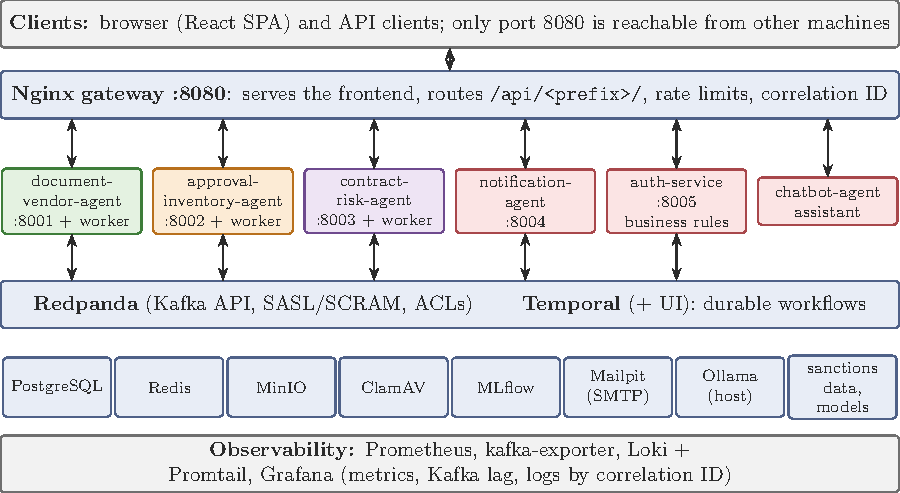
\includegraphics{figures/diagrams/block}
\caption{Block diagram of the deployed system}\label{fig:block}
\end{figure}

\begin{table}[!htbp]
\centering\tablestyle
\caption{Architectural layers}\label{tab:layers}
\begin{tabularx}{\textwidth}{|L{0.19\textwidth}|Y|}
\hline
\textbf{Layer} & \textbf{Components and responsibilities} \\ \hline
Clients & The React application and API clients reach the platform only through the gateway on port 8080. \\ \hline
Gateway & Nginx serves the frontend, routes API paths to the services, limits request rates on authentication endpoints and assigns a correlation ID. \\ \hline
Application services & Document and Vendor agent (8001), Approval and Inventory agent (8002), Contract and Risk agent (8003), notification agent (8004), authentication and business-rules service (8005) and the assistant. Every service checks the JWT and role, except health, metrics and the HMAC-signed webhooks. \\ \hline
Background workers & The document, approval and contract services each run a worker that consumes events, runs Temporal workflows and performs slow tasks such as OCR and model inference. \\ \hline
Messaging and orchestration & Redpanda carries the events with per-service credentials; Temporal runs the approval, reclaim and renewal workflows. \\ \hline
Data and platform services & PostgreSQL holds the records, Redis the reservation locks and rule caches, and MinIO the files. ClamAV scans uploads, MLflow tracks the trained models, Mailpit receives development e-mail, and Ollama runs the assistant's model on the host. \\ \hline
Observability & Prometheus collects metrics, Loki collects logs, and Grafana shows request rates, latency, errors, Kafka consumer lag and the logs of one correlation ID across services. \\ \hline
\end{tabularx}
\end{table}

\subsection{Main Data Paths}
The principal data paths are:
\begin{enumerate}
  \item \textbf{User access:} the browser loads the frontend from Nginx; API calls are routed to the right service after the gateway strips the \texttt{/api/<prefix>/} segment.
  \item \textbf{Document processing:} the Document and Vendor agent checks and scans an upload, stores it in MinIO and publishes \code{document.ingested} through the outbox. Its worker reads, classifies and extracts the document and publishes \code{document.classified} and \code{vendor.matched}.
  \item \textbf{Approval processing:} the Approval and Inventory agent reserves stock, saves the request and starts a Temporal workflow. An approve or reject call signals the workflow; the worker applies the decision, updates the status and publishes \code{approval.decided}.
  \item \textbf{Contract processing:} the Contract and Risk agent generates the contract for an approved request and sends it for signature. When it is signed, \code{contract.signed} moves the request to \emph{ordered}; marking the goods as received makes it \emph{fulfilled}, and the vendor's invoice is matched against it.
  \item \textbf{Risk assessment and notifications:} the Contract and Risk agent publishes risk, renewal and offboarding events; the notification agent consumes them and sends e-mail.
  \item \textbf{Supporting services:} PostgreSQL stores the records (with pgvector for the assistant's index), Redis guards reservations, MinIO stores files, and MLflow records the training runs of the trained models.
\end{enumerate}
Together, these paths show how synchronous API calls, asynchronous events and durable workflows combine to carry a request from intake to completion.

\section{x}\label{sec:code}\label{sec:eval}

% Chapter 6: Conclusion and Future Scope

\chapter{Conclusion \& Future Scope} \label{chap6}
\newpage

This report presented the design and implementation of an Agentic AI-based IT Procurement Intelligence Platform. The study of existing techniques showed that document extraction, clause analysis, approval workflows, anomaly detection and risk scoring are usually treated as separate problems. The project joins them in one event-driven system of four cooperating agents: Document and Vendor Intelligence, Approval and Inventory Intelligence, Contract and Risk Analysis, and a Platform agent for authentication, business rules, notifications and a conversational assistant.

In the implemented system a document arriving by upload, e-mail or a watched folder is scanned, read, classified, extracted, matched to a vendor and confidence-scored; a purchase request is routed through spend-tier approvals with SLA reminders, escalation and race-safe stock reservation; an approved request becomes a contract that is signed in the application after the vendor's risk is shown, read by a legal language model and tracked for renewal; under-used licences are proposed for reclaim with explanations and a grace period; and every vendor carries an explainable risk score with hard overrides and drift monitoring. The whole flow runs through one gateway and is verified by 823 service unit tests, a shared-code suite and four end-to-end suites, all passing at the time of writing.

The design follows one principle throughout: trained models are used only where they measurably beat a simple rule on held-out data, rules remain where certainty and auditability matter, and people stay in control of low-confidence documents, bank-detail changes, licence reclaims, high-risk signatures and model drift. Fail-closed scanning, dual control, separation of duties, HMAC-verified and replay-protected callbacks, role-based access, an audit log and correlation-ID tracing make the platform suitable for a sensitive financial process.

\paragraph{Limitations.}
\begin{itemize}
  \item All training and test data except the CUAD contracts is synthetic, so no accuracy claim is made for an organisation's real documents, licences or vendors.
  \item Field extraction from photographed or scanned images is weak (49\% of fields correct), so such documents depend on human review.
  \item The licence-anomaly model misses most gradual declines and flags a few normal licences; its proposals always need approval.
  \item The review threshold of 0.8 is a heuristic that has not been calibrated against measured error rates.
  \item Adverse-media screening and budget tracking are not built (their business rules are seeded but have no effect), and live GSTIN registry lookups are switched off by default.
  \item Signing happens in the application; the external Documenso and DocuSign clients are not used in the demonstrated configuration and would need the same risk check at send time.
  \item The system runs on a single Docker host: Kafka traffic is not encrypted, development credentials must be rotated before any shared deployment, and the 17 October audit left some issues open, for example logout not revoking the refresh token and a request being committed before its event is staged.
\end{itemize}

\paragraph{Future scope.}
\begin{itemize}
  \item Calibrate the document review gate using evidence from purchase orders and the vendor master, so that the share of documents processed without review is chosen for a target error rate; this is the subject of the team's planned research paper.
  \item Evaluate and improve extraction on real, anonymised procurement documents, for example by fine-tuning LayoutLMv3 on labelled invoices, and retrain the classifier from reviewers' corrections.
  \item Add adverse-media screening (for example with FinBERT), budget tracking, and live GSTIN registry checks with quota management.
  \item Connect an external e-signature provider with the risk acknowledgement enforced at send time.
  \item Close the open audit items, encrypt Kafka traffic, run the test suites in the CI pipeline, and deliver reminder events by e-mail.
  \item Deploy to a managed cloud or Kubernetes environment and measure throughput and latency under load.
\end{itemize}


\cleardoublepage
\phantomsection
\addcontentsline{toc}{chapter}{References}
% References (IEEE style, numbered in order of first citation)
\begin{thebibliography}{99}

\bibitem{smith2007tesseract}
R.~Smith, ``An overview of the Tesseract OCR engine,'' in \emph{Proc. Int. Conf. Document Analysis and Recognition (ICDAR)}, 2007.

\bibitem{cui2025paddleocr}
C.~Cui \emph{et al.}, ``PaddleOCR 3.0 technical report,'' arXiv:2507.05595, 2025.

\bibitem{auer2024docling}
C.~Auer \emph{et al.}, ``Docling technical report,'' arXiv:2408.09869, 2024.

\bibitem{xu2020layoutlm}
Y.~Xu, M.~Li, L.~Cui, S.~Huang, F.~Wei, and M.~Zhou, ``LayoutLM: Pre-training of text and layout for document image understanding,'' in \emph{Proc. ACM SIGKDD Int. Conf. Knowledge Discovery \& Data Mining}, 2020.

\bibitem{huang2022layoutlmv3}
Y.~Huang, T.~Lv, L.~Cui, Y.~Lu, and F.~Wei, ``LayoutLMv3: Pre-training for document AI with unified text and image masking,'' in \emph{Proc. ACM Int. Conf. Multimedia}, 2022.

\bibitem{kreps2011kafka}
J.~Kreps, N.~Narkhede, and J.~Rao, ``Kafka: A distributed messaging system for log processing,'' in \emph{Proc. NetDB Workshop}, 2011.

\bibitem{richardson2018microservices}
C.~Richardson, \emph{Microservices Patterns: With Examples in Java}. Shelter Island, NY, USA: Manning, 2018.

\bibitem{liu2008isolation}
F.~T. Liu, K.~M. Ting, and Z.-H. Zhou, ``Isolation forest,'' in \emph{Proc. IEEE Int. Conf. Data Mining (ICDM)}, 2008.

\bibitem{lundberg2017shap}
S.~M. Lundberg and S.-I. Lee, ``A unified approach to interpreting model predictions,'' in \emph{Proc. Advances in Neural Information Processing Systems (NeurIPS)}, 2017.

\bibitem{chalkidis2020legalbert}
I.~Chalkidis, M.~Fergadiotis, P.~Malakasiotis, N.~Aletras, and I.~Androutsopoulos, ``LEGAL-BERT: The muppets straight out of law school,'' in \emph{Findings of the Association for Computational Linguistics: EMNLP}, 2020.

\bibitem{hendrycks2021cuad}
D.~Hendrycks, C.~Burns, A.~Chen, and S.~Ball, ``CUAD: An expert-annotated NLP dataset for legal contract review,'' in \emph{Proc. NeurIPS Datasets and Benchmarks Track}, 2021.

\bibitem{araci2019finbert}
D.~Araci, ``FinBERT: Financial sentiment analysis with pre-trained language models,'' arXiv:1908.10063, 2019.

\bibitem{apostolo2023legalbertcuad}
\texttt{alex-apostolo/legal-bert-base-cuad}, LEGAL-BERT fine-tuned on CUAD, Hugging Face model repository. [Online]. Available: \url{https://huggingface.co/alex-apostolo/legal-bert-base-cuad} (accessed Oct.~2026).

\bibitem{breiman2001random}
L.~Breiman, ``Random forests,'' \emph{Machine Learning}, vol.~45, no.~1, pp.~5--32, 2001.

\bibitem{yurdakul2018psi}
B.~Yurdakul, ``Statistical properties of population stability index,'' Ph.D. dissertation, Dept. of Statistics, Western Michigan University, 2018.

\bibitem{opensanctions}
OpenSanctions, ``Consolidated sanctions targets,'' dataset, licensed CC BY-NC 4.0. [Online]. Available: \url{https://www.opensanctions.org} (accessed Oct.~2026).

\bibitem{wu2023autogen}
Q.~Wu \emph{et al.}, ``AutoGen: Enabling next-gen LLM applications via multi-agent conversation,'' arXiv:2308.08155, 2023.

\bibitem{pedregosa2011sklearn}
F.~Pedregosa \emph{et al.}, ``Scikit-learn: Machine learning in Python,'' \emph{Journal of Machine Learning Research}, vol.~12, pp.~2825--2830, 2011.

\bibitem{biryukov2016argon2}
A.~Biryukov, D.~Dinu, and D.~Khovratovich, ``Argon2: New generation of memory-hard functions for password hashing and other applications,'' in \emph{Proc. IEEE European Symp. Security and Privacy (EuroS\&P)}, 2016, pp.~292--302.

\end{thebibliography}


\phantomsection
\addcontentsline{toc}{chapter}{Acknowledgement}
% Acknowledgement Page

\begin{centering}
{\LARGE\bfseries Acknowledgement}\\
\end{centering}

\vspace{0.5cm}
\justify
The success of a project like this, which demands technical expertise, patience and generous support from guides, is possible only when team members work together. We take this opportunity to express our gratitude to those who were instrumental in its completion. We thank our project guide \textbf{Dr. Jyoti More} and our external guide \textbf{Mr. Alok Chilka} for their tremendous support and help; without them, this project would not have reached fruition. We also thank our project coordinator \textbf{Dr. Rakhi Kalantri} for regular inputs on documentation and the project timeline, and our Head of Department \textbf{Dr. M. Kiruthika} for her encouragement. Finally, we thank our Principal, \textbf{Dr. S. M. Khot}, and our college, \textbf{Fr. C. Rodrigues Institute of Technology, Vashi}, for the opportunity and the environment to learn and grow.

\vspace{3cm}
\hfill
\begin{tabular}[t]{l@{}}
\textbf{Project Group Members:} \\[1cm]
1. More Anjali Dinesh, 1023207 \\[0.9cm]
\rule{5cm}{0.4pt} \\[0.8cm]
2. Sankaye Vaidehi Jagdeep, 1023239 \\[0.9cm]
\rule{5cm}{0.4pt} \\[0.8cm]
3. Sawant Niraj Ravindra, 1023240 \\[0.9cm]
\rule{5cm}{0.4pt} \\[0.8cm]
4. Shete Anooj, 1023250 \\[0.9cm]
\rule{5cm}{0.4pt}
\end{tabular}


\phantomsection
\addcontentsline{toc}{chapter}{Appendix A: Timeline Chart}
% Appendix A: Timeline Chart

\vspace*{5cm}
\begin{centering}
{\LARGE\bfseries Appendix A: Timeline Chart}\\
\end{centering}

\newpage
\renewcommand{\thefigure}{A.1}

Figure~\ref{fig:gantt} shows the project timeline. The bars up to October 2026 are taken from the dates of the commits in the project repository (113 commits between 4 July and 20 October 2026) and from the dated review and audit records; the bars for November and December are the planned testing and submission phases.

\begin{figure}[!htbp]
\centering
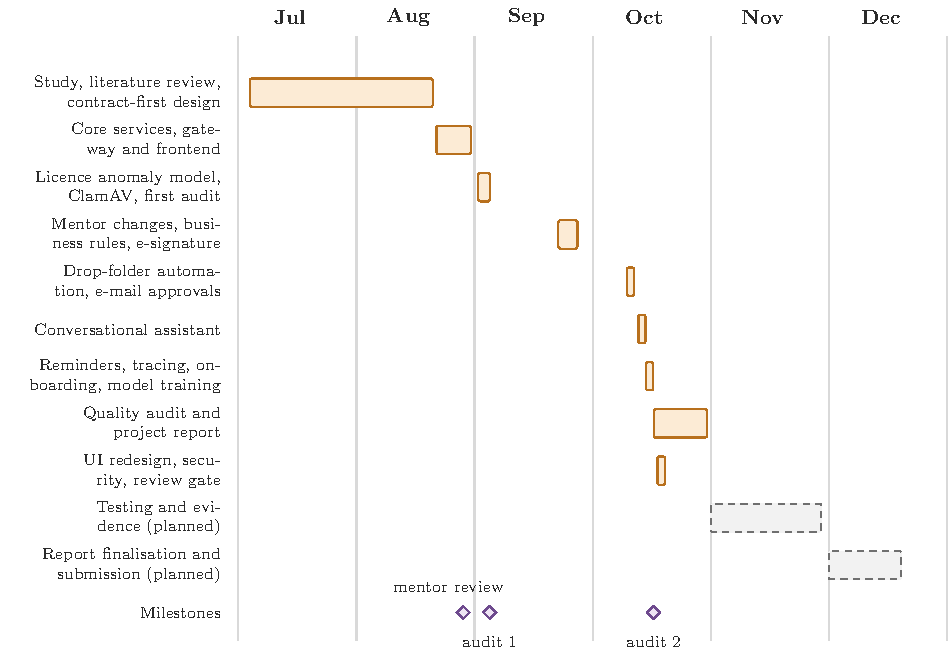
\includegraphics{figures/diagrams/gantt}
\caption[Project timeline]{Project timeline (solid: completed, from the repository history; dashed: planned)}\label{fig:gantt}
\end{figure}


\phantomsection
\addcontentsline{toc}{chapter}{Appendix B: Sustainable Development Goal (SDG) Mapping}
\chapter*{Appendix B}
\label{app:sdg_mapping}

The project team has identified the following Sustainable Development Goals (SDGs) as relevant to the project. The mapping shows the relationship between the project problem, the proposed solution and each selected SDG.

\begin{center}
\textbf{\large SDG Mapping of the Project}
\end{center}

\begin{center}
\tablestyle\small
\begin{tabularx}{\textwidth}{|C{1.1cm}|C{1.2cm}|L{3.4cm}|Y|}
\hline
\textbf{Sr. No.} & \textbf{SDG No.} & \textbf{Complete Name of SDG} & \textbf{Rationale / Contribution of the Project} \\ \hline
1 & 9 & Industry, Innovation and Infrastructure & The platform applies machine learning, event-driven software architecture and workflow automation to a core enterprise process, improving the technological capability and efficiency of IT procurement. \\ \hline
2 & 12 & Responsible Consumption and Production & Duplicate-invoice detection, inventory reservation and reorder suggestions, and the reclaim of under-used software licences reduce wasted purchases and idle resources. \\ \hline
3 & 16 & Peace, Justice and Strong Institutions & Role-based access, separation of duties in approvals, dual control of payment-detail changes, sanctions screening, audit logging and explainable decisions support accountable, transparent and fraud-resistant institutions. \\ \hline
\end{tabularx}
\end{center}

\vspace{0.3cm}
\noindent\textbf{Guidelines for Students:}
\begin{itemize}
  \item Identify only the SDG(s) that have a direct and meaningful connection with the project.
  \item Mention the official SDG number and complete name.
  \item Provide a clear rationale explaining how the project contributes to the selected SDG.
  \item Avoid mapping an SDG merely because the project falls within a particular technology domain.
  \item The SDG mapping should be discussed and validated with the Project Guide.
\end{itemize}

\vspace{1.2cm}
\noindent\begin{tabular}{@{}p{0.5\textwidth}p{0.45\textwidth}@{}}
\rule{5.5cm}{0.4pt} & Name of Project Guide: Dr. Jyoti More \\
Signature of Project Guide & \\[0.6cm]
Date: \rule{3cm}{0.4pt} & \\
\end{tabular}


\phantomsection
\addcontentsline{toc}{chapter}{Appendix C: Complex Engineering Problem Identification and Evaluation}
% Appendix C: Complex Engineering Problem Identification and Evaluation

\chapter*{Appendix C}

\begin{center}
{\large\bfseries Appendix C: Complex Engineering Problem Identification and Evaluation}
\end{center}

\noindent The Washington Accord emphasises the ability of engineering graduates to identify, analyse and solve complex engineering problems using appropriate engineering knowledge, modern tools, multidisciplinary thinking and analytical reasoning. The Major Project provides an opportunity for students to demonstrate these abilities through a structured and evidence-based project.

\vspace{0.2cm}
\noindent This appendix provides a structured mechanism to assess the complexity of the Major Project. The assessment is first carried out by the student team and then verified by the Project Guide.

\section*{A. Project Details}
\begin{center}
\renewcommand{\arraystretch}{1.35}
\begin{tabularx}{\textwidth}{|L{4.2cm}|Y|}
\hline
\textbf{Project Title} & Agentic AI Procurement Solution \\ \hline
\textbf{Group / Team No.} & \todo{team number} \\ \hline
\textbf{Name of Student(s)} & More Anjali Dinesh (1023207), Sankaye Vaidehi Jagdeep (1023239), Sawant Niraj Ravindra (1023240), Shete Anooj (1023250) \\ \hline
\textbf{Project Guide} & Dr. Jyoti More \\ \hline
\textbf{Academic Year} & 2026--2027 \\ \hline
\end{tabularx}
\end{center}

\section*{B. Complexity Evaluation}
\noindent For each parameter, the student team assigns a score from \textbf{0 to 3} with a justification or evidence. The Project Guide reviews the assessment and records the verified score in the final column.

\begin{center}
\tablestyle
\begin{tabularx}{\textwidth}{|C{0.8cm}|L{3.2cm}|C{1.3cm}|Y|C{1.3cm}|}
\hline
\textbf{Sr. No.} & \textbf{Complexity Parameter} & \textbf{Student Score} & \textbf{Student Justification / Evidence} & \textbf{Guide Score} \\ \hline
1 & Problem novelty and research depth & \todo{score} & Integrates document AI, workflows and risk scoring in one governed pipeline; the individual techniques are established (Chapter~\ref{chap2}). & \\ \hline
2 & Multidisciplinary knowledge requirement & \todo{score} & Combines document processing, machine learning, natural language processing, distributed systems, workflow engines, security and web development. & \\ \hline
3 & System design complexity & \todo{score} & Six FastAPI services and three workers in 24 running containers, a shared event and database contract, a transactional outbox, durable workflows and a gateway. & \\ \hline
4 & Technology integration & \todo{score} & FastAPI, Redpanda, Temporal, PostgreSQL, Redis, MinIO, ClamAV, MLflow, Prometheus, Grafana, Loki, Ollama and React in one containerised stack. & \\ \hline
5 & Data analysis and experimentation & \todo{score} & Three models trained and kept only after beating a baseline on held-out data; Legal-BERT evaluated on 102 CUAD test contracts; extraction measured on 15 PDFs and 24 image variants. All training data is synthetic (Section~\ref{sec:eval}). & \\ \hline
6 & Societal / industrial relevance & \todo{score} & Addresses duplicate payments, unused licences and payment-fraud risks that affect organisations. & \\ \hline
7 & Stakeholder involvement & \todo{score} & Four user roles modelled; guidance from an external industry guide and mentor feedback rounds. & \\ \hline
8 & Sustainability considerations & \todo{score} & Reduces wasted purchases and unused licences. & \\ \hline
\multicolumn{2}{|r|}{\textbf{Total Score}} & \todo{total} \textbf{/ 24} & & \textbf{\quad/ 24} \\ \hline
\end{tabularx}
\end{center}

\noindent\textbf{Scoring Guideline:} 0 -- Not applicable / negligible; 1 -- Basic level of complexity; 2 -- Moderate level of complexity; 3 -- Significant / high level of complexity. Maximum score: 24.

\section*{C. Final Project Classification}
\noindent The final classification is based on the score verified by the Project Guide.

\begin{center}
\renewcommand{\arraystretch}{1.3}
\begin{tabular}{|c|L{7cm}|}
\hline
\textbf{Score Range} & \textbf{Project Classification} \\ \hline
0--8 & Simple Engineering Problem \\ \hline
9--16 & Moderately Complex Engineering Problem \\ \hline
17--24 & Complex Engineering Problem \\ \hline
\end{tabular}
\end{center}

\noindent\textbf{Final Classification:}\quad
$\square$ Simple \qquad $\square$ Moderately Complex \qquad $\square$ Complex Engineering Problem

\vspace{1cm}
\noindent\rule{5.5cm}{0.4pt}\hfill Date: \rule{3cm}{0.4pt}\\
Project Guide Signature


\phantomsection
\addcontentsline{toc}{chapter}{Appendix D: Project Outcomes}
% Appendix D: Project Outcomes

\vspace*{5cm}
\begin{centering}
{\LARGE\bfseries Appendix D: Project Outcomes}\\
\end{centering}

\newpage

\section*{Publications and Competitions}
% TODO (team): replace these rows with the final details before submission.
\begin{center}
\tablestyle
\begin{tabularx}{\textwidth}{|L{0.22\textwidth}|Y|L{0.18\textwidth}|}
\hline
\textbf{Outcome} & \textbf{Details} & \textbf{Status} \\ \hline
Research paper & A paper on calibrated, evidence-based review gates for procurement documents (provisional title: \emph{Measuring the Value of Enterprise Context in Selective Automation of Procure-to-Pay Documents}) & In preparation \\ \hline
Project competitions & To be added by the team & -- \\ \hline
\end{tabularx}
\end{center}

\section*{Technical Outcomes}
\begin{itemize}
  \item A working, containerised platform of six services and three workers that takes a procurement document or request from intake to a signed contract, receipt and invoice match.
  \item Three trained models (document classifier, licence-anomaly detector, vendor risk model) and one adopted language model (Legal-BERT for clauses), each kept only after beating a baseline on held-out data (Section~\ref{sec:eval}).
  \item 823 service unit tests, a shared-code suite and four end-to-end suites, with a regression test for every fixed audit finding.
  \item Documentation for reproduction: setup and run scripts, a technical reference, a business-rules register and dated evaluation results.
\end{itemize}


\end{document}
